%%%%%%%%%%%%%%%%%%%%%%%%%%%%%%%%%%%%%%%%%%%%%%%%%%%%%%%%%%%%%%%%%%%%%%%%%%%%%%%
%%	PARA INSERTAR FIGURAS USAR LA FUNCION PREDEFINIDA \imagen
%%
%%      \imagen{escala}{path imagen}{caption}{referencia}
%%
%% donde:
%% 	* escala: es un valor numérico. Preferentemente usar valores entre 0 y 1.
%%		(ejemplo: 0.2)
%% 	* path: imagen es el directorio relativo donde se encuentra la imagengit
%%		(ejemplo: Figures/Logos/conae-logo.png)
%%	* caption: texto de pie de figura.
%%	* referencia: texto que sirve para citar la figura.
%%		(ejemplo: fig:conaelogo) luego se podrá hacer referencia \ref{fig:conaelogo}
%%%%%%%%%%%%%%%%%%%%%%%%%%%%%%%%%%%%%%%%%%%%%%%%%%%%%%%%%%%%%%%%%%%%%%%%%%%%%%%

%------------------------------------------------------------------------------
% Formato del documento
\documentclass[11pt, a4paper, twoside]{report}

%------------------------------------------------------------------------------
% TEMPLATE MDIAE (ACÁ SE ENCUETRAN LAS CUSTOMIZACIONES)
% Remitirse al archivo mdiaedoc.sty
\usepackage{mdiaedoc}

%Configuración de los márgenes
\usepackage[top=3cm, bottom=3cm, left=2.5cm, right=1.5cm]{geometry}

\usepackage{natbib}
%\usepackage[natbibapa]{apacite} 
\usepackage{import}

% Para gráficos
% \usepackage{tikz}
% \usetikzlibrary{shapes,snakes}
% \usetikzlibrary{arrows,positioning}
% \usetikzlibrary{babel}

%pagina en blanco
\usepackage{afterpage}

%Para agregar notas
\usepackage{todonotes}

% For comment
\usepackage{comment}

% For appendix
\usepackage{appendix}

% For epigraph
\usepackage{epigraph}

% For rotate image
\usepackage{rotating}

% For add coding
\usepackage{listings}

\usepackage{graphicx}

\usepackage{longtable}

\usepackage{lipsum} % just for dummy text- not needed for a longtable

%------------------------------------------------------------------------------
% Esto no se usa (YA ESTA DEFINIDO EN EL TEMPLATE)
%\usepackage{setspace}

%%%%%%%%%%%%%%%%%%%%%%%%%%%%%%%%%%%%%%%%%%%%%%%%%%%%%%%%%%%%%%%%%%%%%%%%%%%%%%%
% COMIENZO DEL DOCUMENTO
%%%%%%%%%%%%%%%%%%%%%%%%%%%%%%%%%%%%%%%%%%%%%%%%%%%%%%%%%%%%%%%%%%%%%%%%%%%%%%%
\begin{document}

\makeatletter
\author{Arias Emmanuel}
\makeatother

%------------------------------------------------------------------------------
% PORTADA
\portadatesis{Diseño de una arquitectura de aviónica tolerante a fallas basada en componentes COTS para vehículos
satelitales de nueva generación}{Arias Emmanuel}{UNIVERSIDAD NACIONAL DE LA MATANZA}{Buenos Aires,
2018}{2018}{Gustavo Wiman}{INVAP, Bariloche, Provincia de Rio Negro}

\pagenumbering{gobble}


%------------------------------------------------------------------------------
% EN CASO DE TENER UN ASESOR CIENTIFICO, DESCOMENTAR LO SIGUIENTE
% \begin{center}
% \normalsize ASESOR CIENTÍFICO:\\
% \normalsize \textit{\textbf{Nombre del asesor}}\\
% \end{center}

%------------------------------------------------------------------------------
% COMPLETAR CON LICENCIA CREATIVE COMMONS SEGÚN CORRESPONDA
%\begin{center}
%%%%% Ejemplo %%%%%%
%\begin{figure}[H] \centering \includegraphics[width=3cm,
%    keepaspectratio=true]{imagenes/Logos/creativecommons.png} \end{figure} \vspace*{-0.5cm}
%    Esta obra está bajo una
%    \href{http://creativecommons.org/licenses/by-sa/2.5/ar/}{Licencia
%    Creative Commons Atribución-CompartirIgual 2.5
%    Argentina.}  \end{center}

\newcommand\blankpage{%
	\null
	\thispagestyle{empty}%
	\addtocounter{page}{-1}%
	\newpage}

\afterpage{\blankpage}

\newpage
Parte de los resultados obtenidos en el presente trabajo
fueron presentados en el \textit{Congreso Argentino de Tecnologías
  Espaciales 2017 (Córdoba, Argentina)}, bajo el título:
\textit{Estudio de la confiabilidad de arquitecturas tolerantes a fallas
basada en componentes COTS para aviónicas de vehículos
espaciales}
\newpage

\chapter*{}
\begin{flushright}
  \textit{
    A mi madre, \\
    gracias a tus palabras \\
    mirá a dónde llegué. Y no me detendré. 
  }
\end{flushright}

\chapter*{Abstract}
\label{chap:abstract}
The space missions development involves costs of major magnitude, the most important costs
being the development, and the materials used for the manufacture of satellites. The high
cost of these materials is because they are manufactured exclusively for their application
to space activity, that mean that they are "qualified to fly." There are other components
called COTS (Commercial Off-The-Shelf). These COTS components are considerably more
economical than the "classic" ones, thus helping to significantly reduce costs. This is
important to the Argentinian space industry. To achieve a correct application of these
components, it is necessary develop  techniques, strategies and architectures that ensure
that the probability of catastrophic failure and degradation are compatible with the mission.
In this work, we firstly studied and proposed models of different topologies that will
be used to develop a fault tolerant architecture based on COTS components. Then, a communication
protocol called CANae is developed. CANae is  based on the CAN (Controller Area Network)
protocol, and CANae is oriented to work in distributed networks. Finally, in this thesis
be proposed an architecture based on both COTS components and distributed networks, that
uses the protocol CANae for the communication with its components. In this way, an
architectural proposal is developed to ensures that the system is reliable, even though
the components that make it up are of low reliability.


\textbf{Keywords: COTS Components, Fault Tolerant Architecture, Avionics, Fault Tolerance, Satellites}

\chapter*{Resumen} % si no queremos que añada la palabra "Capitulo"
%\addcontentsline{toc}{chapter}{Resumen} % si queremos que aparezca en el índice

Esta tesis se trata de
\chapter*{Agradecimientos}
\label{chap:agradecimientos}
%\addcontentsline{toc}{chapter}{Agradecimientos}
Muchas gracias
 %% OPCIONAL
\chapter*{Organizacion de la tesis}
\label{chap:organizacion}
%\addcontentsline{toc}{chapter}{Agradecimientos}

Este trabajo de tesis está organizado de manera tal que, el lector logre comprender
cuál es la problemática que se plantea el autor, conozca el sustento
teórico sobre los cuales la tesis se apoya, y con ello,  y de manera natural, se logre
entender el significado y la importancia de la propuesta de la arquitectura diseñada
en esta tesis.

En el Capítulo \ref{chap:intro} (página \pageref{chap:intro}) se centra en que el lector
entienda la motivación (Sección \ref{chap:motivacion} página \pageref{chap:motivacion})
que impulsan este trabajo de investigación y desarrollo, como así también las
hipótesis (Sección \ref{sec:hipotesis} página \pageref{sec:hipotesis}), objetivos
(Sección \ref{sec:objetivos} página \pageref{sec:objetivos}), objetivos específicos
(Sección \ref{sec:objetivos_especificos} página \pageref{sec:objetivos_especificos}) y las
preguntas de investigación (\ref{sec:preguntas_investigacion} página \pageref{sec:preguntas_investigacion}) que el autor se propone resolver.

En el Capítulo \ref{chap:marco_teorico} (página \pageref{chap:marco_teorico})
En este capítulo se introduce al lector a la teoría en la cual se basa este trabajo de tesis. Entre
las secciones más importantes que se verán se puede mencionar, que en la
Sección \ref{sec:terminologia} (página \pageref{sec:terminologia}) se explica brevemente la
terminología que se utiliza a lo largo de este trabajo. Es importante leer esta sección ya que
algunos términos pueden considerarse sinónimos en el habla común, pero en esta tesis, tienen
significados bien diferenciados.
En la Sección \ref{sec:fiabilidad_software} (página \pageref{sec:fiabilidad_software}) explica
qué es la fiabilidad aplicada en sistemas (de software) y cómo se puede clasificar la fiabilidad. En
Sección \ref{sec:impedimentos} (página \pageref{sec:impedimentos}) se detalla el concepto de los
impedimentos de la fiabiliad, cuáles son los orígenes de las fallas, los modos comúnes de fallas
y las fallas en el software.
La tolerancia a fallas, el núcleo de este trabajo, se explica en la Sección \ref{chap:FaultTolerance}
(página \pageref{chap:FaultTolerance}). En esta sección se detalla el signficado de la tolerancia
fallas, importante para entender este trabajo de tesis.
En la Sección \ref{sec:protocolos_comunicacion} (página \pageref{sec:protocolos_comunicacion})
se brinda un resúmen teórico de diferentes protocolos de comunicación existentes en la actualidad.
En la Sección \ref{seccion:ProtocoloCAN} (página \pageref{seccion:ProtocoloCAN}) se detalla el
protocolo CAN que es utilizado como principal protocolo de comunicación. La arquitectura propuesta
en este trabajo de tesis utiliza un protocolo de comunicación basado en CAN. En esta sección se describe capa física (página \pageref{subsec:capafisca}), capa de enlace (página \pageref{subsec:capa_enlace}), formato del mensaje (página \pageref{subsec:formato_mensaje}) y se comenta sobre un protocolo basado en CAN que es utilizado en aplicaciones de aeronáutica llamado CANAerospace (página \pageref{subsec:CANaerospace})

En el Capítulo \ref{chap:estado_del_arte} (página \pageref{chap:estado_del_arte})




\tabladecontenidos

\chapter*{Lista de acrónimos}
\label{chap:acronimos}
\begin{acronym}[TESIS]
\acro{SW}{Software}
\acro{FT}{Tolerancia a Fallas}
\acro{FA}{Evitación de Fallas}
\acro{FR}{Eliminación de Fallas}
\acro{FF}{Predicción de Fallas}
\acro{MTBF}{Tiempo Medio Entre Fallas}
\acro{MTTF}{Tiempo Medio de Fallas}
\acro{MTTR}{Tiempo Medio de Reperación}
\acro{CMF}{Modo Común de fallas}
\acro{FDIR}{Detección, Aislación y Recuperación de Fallas}
\acro{CONAE}{Comisión Nacional de Actividades Espaciales}
\acro{UNLAM}{Universidad Nacional de La Matanza}
\acro{INVAP}{Investigación Aplicada}
\acro{NASA}{National Aeronautics and Space Administration}
\acro{COTS}{Commercial Off-The-Shelf}
\end{acronym}


%-------------------------------------------------------------------------------
%TODO: Elminiar esta tabla antes de enviar a corregir
%-------------------------------------------------------------------------------
%\listoftodos


%------------------------------------------------------------------------------
% Numeración arábiga a partir de este punto
\pagenumbering{arabic}
\setcounter{page}{1}
\section{Introducción}
Los proyectos aeroespaciales emplean una arquitectura de aviónica que se denomina \textbf{federada}, en la cual cada computadora del sistema se diseña para que desarrolle una sola función específica \citep{Loveless15}. Esta estrategia de diseño tiene varias ventajas, por tal motivo ha sido utilizada a lo largo de los años. En contraposición, cuenta con varias desventajas, que alientan al surgimiento de nuevas formas de pensamiento y desarrollo de aviónica de sistemas espaciales. Algunas de estas desventajas que ya fueron mencionadas con anterioridad son la masa y una utilización ineficiente de los procesadores. Para ello se está comenzando a desarrollar arquitecturas con el paradigma IMA.


% Marco Teorico
\chapter{Marco Teórico}\label{chap:marco_teorico}
\epigraph{Solo sé que no sé nada}{Platón}
% section that talk about terminology
% esta seccion habla sobre los términos importantes a utilizar a lo largo de la tesis
\section{Terminología}\label{sec:terminologia}
Existe una importante diferencia entre los significados de las palabras falla, error y
avería\footnote{En inglés: fault, error y failure.}, que es importante destacar. Teniendo en cuenta 
el Diccionario de Cambridge \citep{CambridgeDictionary}\footnote{\texttt{{https://dictionary.cambridge.org/}}}
el significado de fault es, ``1. something that is wrong with something; 2. an imperfection, something wrong;
3. a mistake, especially something for which you are to blame'', 
que se adapta de mejor manera con la palabra española ``falla'', que según la Real Academia Española \citep{RAE}\footnote{\texttt{{http://www.rae.es/}}} es, ``1. defecto o falta; 2. incumplimiento de una
obligación''.  Por otro lado, Failure según \cite{CambridgeDictionary} es, ``1. the fact of someone or something not succeeding; 2. the fact of not doing something that you must do or are expected to do'', que 
nuevamente se adapta mejor con la palabra española ``avería'', la cual significa: ``1. Daño que impide el funcionamiento de un aparato, instalación, vehículo, etc.'' Por esto, en esta obra se utilizan las palabras: falla, error y avería, para las traducciones de fault, error y failure.

Una \textbf{avería} de sistema ocurre cuando el servicio prestado por el sistema ya no coincide con
las especificaciones del mismo \citep{Hanmer07}. Esto quiere decir que existe un problema que tiene
una consecuencia negativa en el sistema completo, logrando que este ya no logre cumplir con sus
especificaciones. Cuando el sistema no se comporta de la manera que es especificada, este ha
fracasado. Esto significa que lo que se espera de un sistema se encuentra descripto, comúnmente en
especificaciones o requerimientos \citep{Pullum01}.

Para la \cite{IEEE610.12} avería es ``la inhabilitación de una sistema o componente a llevar a
cabo las funciones requeridas en los requerimientos específicos de perfomance del mismo''.

\cite{Hanmer07} ejemplifica averías de sistemas cuando: el sistema se bloquea y se detiene cuando no
debería hacerlo, el sistema calcula un resultado incorrecto, el sistema no está disponible, o el
sistema es incapaz de responder a la interacción con el usuario. Cuando el sistema no hace lo que
debe hacer, el sistema ha fracasado. Las averías son detectados por los usuarios mientras usan el
sistema.

Las averías son causados por los errores. Un \textbf{error} es una parte del estado del sistema
que es susceptible de provocar un avería en el sistema. Un error que afecta al servicio, es una
indicación de que una avería se ha producido \citep{Hanmer07}. Un error se puede propagar, es decir
dar a lugar otros errores \citep{Pullum01}.

\cite{IEEE610.12} define error como ``la diferencia entre un valor computado, observado o medido,
con el valor verdadero, especificado o el teóricamente verdadero''.

Según \cite{Rani11} un error es la parte de estado del sistema que puede conducir a una avería, es una
etapa intermedia entre fallas y averías.

Los errores se pueden clasificar en dos tipos: errores de tiempo y valores \citep{Hanmer07}. Los
errores de valores son aquellos que se manifiestan como valores discretos incorrectos o estados del
sistema incorrecto. En cambio, los errores de tiempo pueden incluir aquellos que no cumplen con el total de las tareas.

\cite{Hanmer07} especifica los siguiente casos más comunes de errores:
\begin{itemize}
 \item Timing: existe una falta de sincronización en la comunicación de los procesos.
 \item Bucles infinitos: ejecución de un bucle sin detenerse, esto consume memoria, y la
avería del sistema.
 \item Error de protocolo: errores en el flujo de comunicación ya que no coinciden los
protocolos. Mensajes enviados en formato diferente, en tiempos diferentes, a lugares de sistemas
incorrectos.
 \item Inconsistencia de datos: los errores son diferentes en diferentes lugares.
 \item Sobrecarga de sistema: el sistema es incapaz de hacer frente a la sobrecarga de
actividades a la que es expuesta.
\end{itemize}

La causa adjudicada o la hipótesis de un error es una \textbf{falla}, también llamado ``bugs''. Una
\textbf{falla activa} es aquella que produce un error \citep{Pullum01}. Una falla es un defecto que está
presente en el sistema y que puede causar un error \citep{Hanmer07}. Es la desviación actual de lo
correcto \citep{Hanmer07} \citep{Rani11}. 

Según \cite{IEEE610.12} una falla es ``un defecto en un dispositivo de hardware o componente; como
por ejemplo un corto circuito o un cable cortado''. También realiza una segunda definición diciendo
que falla es ``un paso incorrecto, proceso, o definición de dato en un programa de computadora''
\citep{IEEE610.12}. Esta última afirmación es la que se usa en el ámbito de este trabajo.

Se puede indicar que un software contiene falla, si dado un conjunto de entradas, se obtienen
resultados que son incorrectos. Una falla es una parte del software, y puede ser eliminada mediante 
la corrección de dicha parte. \citep{XIE}

Debe realizar la distinción entre fallas activas y pasivas. Las primeras son aquellas que han sido descubiertas por algún, es decir, mediante testing o durante el funcionamiento del sistema. Si el sistema no es capaz de identificar la falla, aislar y recuperarse de esta, podría llegar a convertirse en una avería. Por otro lado, las fallas pasivas son aquellas que se encuentran dentro del sistema, pero todavía no ha sido detectada, es decir, que no causa ningún efecto observable eternamente (a nivel de sistema). Debe aclararse que una falla se manifieste o no, depende de lo que esté sucediendo en le sistema y su entorno. 

Algunas fallas introducidas en el \ac{SW} se detallan en \cite{Hanmer07}, lo cual señala que
pueden incluir:
\begin{itemize}
 \item Especificaciones incorrecta de requerimientos
 \item Diseño incorrecto
 \item Errores de programación
\end{itemize}


Resumiendo, la principal diferencia entre falla (fault) y avería (failure) es que la primera, es 
la causa de la segunda. Debido a la existencia de una falla, las entradas del módulo (o sistema) software
que contiene dicha falla, provocará como salida valores y/o resultados incorrectos, es decir, 
que no corresponden con los valores teóricos. Por otro lado una avería, es la consecuencia de una falla, 
y se refiere a cuando el sistema deja de responder o comportarse como debería hacerlo, desviándose 
de sus requerimientos. 

Entonces, como lo indica \cite{Pullum01} con la tolerancia a fallas, lo que se busca es prevenir la
avería mediante la ``tolerancia'' de fallas, las cuales son detectables cuando un error aparece.
Las fallas son el motivo de errores y los errores son motivos de avería \citep{FTDesign}.

También se suele utilizar el término anomalía en las operaciones de vehículos espaciales para
referirse a comportamientos anómalos o no esperados del sistema \citep{SpaceSystemFailures}

En \cite{FTDesign} se describe un ejemplo para diferenciar correctamente estos conceptos. Se considera
el \ac{SW} de una planta nuclear, en la cual existe una computadora que es responsable de controlar
la temperatura, la presión y demás variables de interés para la seguridad del sistema. Se da el
caso de que uno de los sensores detecta que la turbina principal se encuentra girando a una
velocidad menor a la correcta. Esta falla hace que el sistema envíe una señal para aumentar su
velocidad (error). Esto produce un exceso de velocidad en la turbina, lo cual tiene como
consecuencia que la seguridad mecánica apague la turbina. En esta situación el sistema no está
generando energía. Esto se considera un avería, porque el sistema no está entregando el servicio
según lo establecido por los requerimientos. Pero es un avería salvable.

Otro concepto es el de \textbf{mantenibilidad}, esta es la capacidad de un sistema, bajo condiciones normales, de ser restaurado a un estado en el cual puede realizar sus funciones requeridas, cuando se realiza el mantenimiento \citep{Rausand04}.

En secciones posteriores se ven los conceptos de confiabilidad, disponibilidad y seguridad (Sección \ref{subsec:confiabilidad}, \ref{subsec:disponibilidad}, \ref{subsec:seguridad}, respectivamente).


% Section that talk about dependability on software
% TODO:La fiabilidad en el software
\section{La fiabilidad en el software}\label{sec:fiabilidad_software}
El objetivo final de la \ac{FT}, es el desarrollo de un sistema fiable \citep{FTDesign}. Teniendo
en cuenta que el \ac{SW} que se encuentra dentro de las naves espaciales, como satélites,
lanzadores, y sobre todo vehículos tripulados son críticos, ya que de ellos dependen el éxito o
fracaso de una misión o la vida de seres humanos,y por lo tanto, se debe llevar a cabo un sistema fiable.
La fiabilidad de un sistema es la capacidad del mismo de entregar a los usuarios un nivel
deseado de servicio \citep{FTDesign}.

La fiabilidad también se la puede considerar como una propiedad global que permite justificar la
confianza de los servicios de un sistema \citep{FTAvionics}. Por lo tanto, como lo indica
\cite{FTAvionics} la fiabilidad es un término amplio y cualitativo que está relacionado con
atributos no funcionales (o ``-ilities''), que buscan generar un sistema ``ideal'', especialmente
cuando su funcionamiento es crítico.

Como se muestra en la Figura \ref{fig:dependability_relations} la consecuencia de la fiabilidad es
la relación entre la evitación de fallos y la reducción de fallos, así como también la \ac{FT}.

\begin{figure}[h]
 \centering
 \includegraphics[scale=0.5]{images/Marco_teorico/dependability_relations}
  \caption{Fiabilidad \protect\citep{FTAvionics}}
\label{fig:dependability_relations}
\end{figure}

Según \cite{Pullum01} la fiabilidad puede ser clasificada en:
\begin{itemize}
 \item Impedimentos: son aquellas cosas que se interponen en el camino de la fiabilidad. Son las
fallas, errores y averías.
 \item Medios: los medios para lograr la fiabilidad, según el autor, se pueden dividir en dos
grupos:
  \begin{enumerate}
    \item Aquellos que son utilizados durante la construcción del \ac{SW} (\ac{FA}\footnote{En
    inglés, Fault Avoidance} y \ac{FT}).
    \item Aquellos que contribuyen con la validación del \ac{SW} una vez desarrollado
    (\ac{FR}\footnote{En inglés, Fault Removal} y \ac{FF}\footnote{En inglés, Fault Forecasting}).
  \end{enumerate}

 \item Atributos: describen las propiedades de la fiabilidad y proporcionan una forma de evaluar el
logro de esas propiedades.
\end{itemize}

% TODO: deteriodo de la confiabilidad
\section{Impedimentos de la confiabilidad}\label{sec:impedimentos}
El impedimento de la confiabilidad o deterioro de la confiabilidad es definido en términos de
fallas, errores, y avería \citep{FTDesign}. Los mismos fueron desarrollados en la sección
\ref{sec:terminologia}. Lo que tienen en común estos tres conceptos, es que avisan, o dan alerta
cuando algo está mal \citep{FTDesign}. La diferencia radica, en que las fallas son a nivel físico;
los errores se dan a nivel computacional; mientras que las averías se dan a nivel de sistema
\citep{FTDesign}.

\subsection{Orígenes de la falla}
Existen diversos orígenes de fallas. Estas pueden provenir desde terceros, en el caso de productos
comprados, pueden deberse a una falta del conocimiento del problema, falta de tiempo, etc.
\cite{FTDesign} clasifica el origen de las fallas en cuatro grupos: \textit{especificación
incorrecta, implementación incorrecta, defectos de fabricación y factores externos}

Las \textit{especificaciones incorrectas} son aquellas que surgen debidas a una incorrecta
especificación de requerimientos o un mal diseño de una arquitectura o de un algoritmo
\citep{FTDesign}. Estos orígenes de fallas son bastante comúnes en el desarrollo de sistemas. Un
ejemplo típico citado por \cite{FTDesign}, es el caso de requerimientos que ignoran aspectos del
medio ambiente en el que opera el sistema. Una mala redacción de un requerimiento o el olvido de
uno de ellos, puede traer graves problemas, atrasos y pérdida de dinero,  en el diseño y producción
de un sistema espacial.

Las \textit{implementaciones incorrectas}, se refieren a las \textit{fallas de diseño}, surgen
cuando el sistema implementado no cumple con los requerimientos \citep{FTDesign}.

Otro orígen de falla son los \textit{defectos de los componentes} \citep{FTDesign}.Estos pueden
incluir defectos de fabricación, defectos aleatorios dados en los componentes, etc.

Y por último se tienen las fallas que son causadas por \textit{factores externos}, los cuales
provienen del medio ambiente, usuarios u operadores \citep{FTDesign}. Ejemplos de estos factores
externos pueden ser, vibraciones, cargas electroestáticas, temperatura, radiación electromagnética,
envío incorrecto de comandos, etc.

% TODO: Modos comúnes de fallas
\subsection{Modos comúnes de fallas}
Un \textit{\ac{CMF}}\footnote{En inglés, common-mode faults} es una falla que ocurre
simultáneamente en dos o más componentes redundantes \citep{FTDesign}.

\cite{Gangloff75} define los \ac{CMF} como múltiples unidades de fracaso debido a una sola causa.

\ac{CMF} son causados por fenómenos que crean dependencias entre unidades redundadas, lo que causa
la falla de estas unidades simultáneamente \citep{FTDesign}.

Según como lo indica \cite{FTDesign} el único enfoque para combatir los \ac{CMF}, es mediante el
diseño en diversidad. Diseño en diversidad es la implementación de más de una variante de la
función en cuestión \citep{FTDesign}. Esto se puede lograr variando los algoritmos que se utilizan,
diferentes equipos de trabajo realicen las mismas partes del sistema, de manera tal de tener
redundancia en código, etc.

\subsection{Falla de causa común}
Una falla de causa común (CCF) se define como cualquier instancia donde múltiples unidades o elementos fallan
debido a una causa común. Estos tipos de fallas pueden ocurrir debido al diseño de los equipos, catástrofes externas, fuentes de energías compartidas, la utilización de equipamientos provenientes de un mismo fabricante, etc. \citep{Rani11}

%TODO: Fallas en el Software
\subsection{Fallas en el Software}
El \ac{SW} difiere en gran medida con el \ac{HW}. En primer lugar el \ac{SW} no envejece, no se deforma, tampoco se puede quebrar ni ser afectado por el medio ambiente. Debido a que esta obra tiene como área de estudio el software de vuelo de satélites, se asume que el \ac{SW} es determinístico, esto quiere  decir que tendrá el mismo comportamiento, en las mismas circunstancias, al menos que exista un problema en el \ac{HW} (provocado por el ambiente espacial, por ejemplo).

El \ac{SW} es determinístico, siempre responde de la misma manera en el mismo ambiente, a menos que falle.

Por otro lado, el \ac{SW} se lo puede actualizar varias veces a lo largo del su ciclo de vida.

En tercer lugar, arreglar bugs de \ac{SW} \textbf{no significa que el mismo sea más confiable}, al contrario pueden ocurrir nuevos errores \citep{FTDesign}.

Por último el \ac{SW} es mucho más complejo y menos regular que el \ac{HW}. Tests tradicionales y métodos de debug pueden ser inadecuados para los sistemas de \ac{SW}

% TODO: medios de fiabilidad
\section{Medios de fiabilidad}\label{sec:medios_falla}
Los medios de confiabilidad son métodos y técnicas que permiten el desarrollo de un sistema
confiable \citep{FTDesign}. Los medios se pueden dividir en dos grandes grupos \citep{Pullum01}:
\begin{enumerate}
 \item Aquellos que son empleados durante el proceso de construcción del \ac{SW},
 \item y aquellos que ayudan en la validación del \ac{SW} después que fue desarrollado.
\end{enumerate}

Dentro del primer grupo se tiene:
\begin{itemize}
 \item \acl{FA}
 \item \acl{FT}
\end{itemize}

Por otro lado, en el segundo grupo se puede mencionar los siguientes:
\begin{itemize}
 \item \acl{FR}
 \item \acl{FF}
\end{itemize}

\subsection{\acl{FA}}
\ac{FA} son técnicas de mejoramiento de la fiabilidad utilizadas durante el desarrollo de \ac{SW}
para reducir el número de fallas introducidas durante la etapa mencionada \citep{Pullum01}. Estas
técnicas pueden estar presentes en las especificaciones y requerimientos del sistema, métodos de
diseño de \ac{SW} \citep{Pullum01}.

\cite{FTDesign} la denomina \textit{prevención de fallas}\footnote{En inglés, Fault prevention}, y
coincide con el autor anterior, definiendo \ac{FA} como técnicas de control de calidad durante la
especificación y fabricación de los procesos de diseño.

% In page 22 of Pullum01 there're more definitions that may be important inside Failure avoidance

\subsection{\acl{FT}}
En la sección~\ref{chap:FaultTolerance} (página~\pageref{chap:FaultTolerance}) se discute con
mayor detalle la \ac{FT}.

\subsection{\acl{FR}}
La \ac{FR} hace referencia a las técnicas utilizadas para mejorar la fiabilidad empleadas durante
la validación y verificación del \ac{SW} \citep{Pullum01}. Estas técnicas mejoran la fiabilidad del
\ac{SW} mediante la detección de fallas, usando métodos de verificación y la validación, y
eliminando las fallas que se van detectando \citep{Pullum01}.

Por otro lado \cite{FTDesign} indica que el \ac{FR} se lleva a cabo durante fases de desarrollo de
\ac{SW} tanto como durante el ciclo de vida de un sistema. Durante la fase de desarrollo, \ac{FR}
consiste en tres pasos: \textit{verificación, diagnóstico y corrección} \citep{FTDesign}. \ac{FR}
durante la vida operacional de un sistema, consiste en el mantenimiento preventivo y correctivo del
mismo \citep{FTDesign}.

\subsection{\acl{FF}}
La \ac{FF} se realiza mediante la realización de una evaluación del comportamiento del sistema con
respecto a la ocurrencia o la activación de una falla. Según \cite{FTDesign} esta evaluación puede ser:
\begin{itemize}
 \item Cualitativa: que tiene como objetivo clasificar los modos de fallas o combinaciones de
eventos que llevan a la avería del sistema,
 \item Cuantitativa: que tiene como objetivo evaluar en término de probabilidad, el grado en el
cual los atributos de fiabilidad son satisfechos.
\end{itemize}

\ac{FF} incluye técnicas para aumentar la fiabilidad del sistema que son usados durante la
validación del \ac{SW}, con el objetivo de estimar la presencia de fallas y la ocurrencia o
consecuencia de fracasos \citep{Pullum01}

% TODO: atributos de la fiabilidad
\section{Atributos de la fiabilidad}\label{sec:atributos_de_la_fiabilidad}
Como se mencionó anteriormente, la fiabilidad de un sistema es la capacidad del mismo de entregar a los usuarios un nivel
deseado de servicio \citep{FTDesign}.

La fiabilidad es una medida de calidad  que abarca los conceptos de confiabilidad, disponibilidad y seguridad \citep{SoftwareFaultToleranceATutorial}. Estos se denominan atributos de la fiabilidad, los cuales son mencionados a continuación.

\subsection{Confiabilidad}\label{subsec:confiabilidad}
La confiabilidad es la probabilidad de que un sistema continúe operando correctamente durante un
intervalo de tiempo dado \citep{SoftwareFaultToleranceATutorial}.

\cite{FTDesign} coincide que la confiabilidad \textit{R(t)}\footnote{En inlgés, Reliability} de un
sistema es la probabilidad de que el sistema opere sin averías en el intervalo de tiempo
\textit{[0,t]}.

La confiabilidad es una medida de la entrega correcta del servicio que brinda un sistema
\citep{FTDesign}.

En sistemas críticos como el \ac{SW} de vehículo espacial, es sumamente necesario que tenga una
alta tasa de confiabilidad, ya que por ejemplo, perder el contacto con la nave, podría representar
la pérdida de la misión, o una gran cantidad de datos. Otro ejemplo que se puede mencionar es de un
satélite geoestacionario de comunicación, la pérdida de este servicio debe ser baja, casi nula
(idealmente).

Coincidiendo, \cite{pressman01} define la confiabilidad como la ``probabilidad de tener operaciones
libre de fallas de un programa de computadora, en un ambiente específico para un tiempo específico''. 

La \cite{IEEE610.12} define confiabilidad como ``La capacidad del sistema o componente de realizar
sus funciones requeridas bajo las condiciones establecidas durante un período de tiempo
especificado''.

\subsection{Disponibilidad}\label{subsec:disponibilidad}
Es la probabilidad de que el sistema esté operando correctamente en un determinado instante de
tiempo \citep{SoftwareFaultToleranceATutorial}. La disponibilidad \textit{A(t)} de un sistema en el
instante de tiempo \textit{t} es la probabilidad que el sistema esté funcionando correctamente en
el instante \textit{t} \citep{FTDesign}.

\cite{FTDesign} realiza un definición matemática de \textit{A(t)}, llamándola también como
\textit{punto de disponibilidad} o \textit{disponibilidad instantánea}. Y la define como:

$$A(T) = \frac{1}{T} \int_0^T \! A(t) \, \mathrm{d}x $$

Para \cite{Hanmer07} la disponibilidad del sistema es el porcentaje de tiempo en el que es capaz de
llevar a cabo una función determinada.

Para el caso de los sistemas que no pueden ser reperados el punto de disponibilidad es igual a la
confiabilidad del sistema \citep{FTDesign}.

Los estados de disponibilidad pueden ser representados en términos de fuera de servicio por año. En
la Tabla \ref{table:avalVSdowntime} que expone \cite{FTDesign} se puede observar esta relación.

\begin{table}[h]
  \centering
  \begin{tabular}{l|l}
    \hline
    Disponibilidad & Fuera de servicio \\ \hline
    90\%           & 36.5 días/año     \\
    99\%           & 3.65 días/año     \\
    99.9\%         & 8.76 horas/año    \\
    99.99\%        & 52 minutos/año    \\
    99.999\%       & 5 minutos/año     \\
    99.9999\%      & 31 segundos/año   \\ \hline
  \end{tabular}
  \caption{Disponibilidad en relación con su baja de servicio por año. Tabla
modificada de \protect\cite{FTDesign}}
  \label{table:avalVSdowntime}
\end{table}

La \cite{IEEE610.12} define la disponibilidad como ``El grado en el cual un sistema o
componente se encuentra operativo y accesible cuando se requiere su uso. También es expresado en
términos de probabilidad''

En satélites de órbita baja (LEO\footnote{Del inglés, Low Earth Orbit}), es necesario que el
satélite se encuentre disponible al momento de su pasada por las estaciones terrenas, con el fin de 
descargar los datos que se fueron almacenando. Del mismo modo, el satélite debe estar disponible
para llevar a cabo las funciones necesarias, y con esto cumplir con su misión (como por ejemplo la
registración de imágenes en una determinada zona terrestre).

Diferente es el caso para los satélites geoestacionarios, ya que estos deberían estar disponible la
mayor parte del tiempo, ya que en la mayoría de los casos son de comunicación.

Resumiendo, la disponibilidad es la probabilidad de que el sistema esté operando correctamente en el instante de tiempo en el que se requiera su servicios, es decir, en el momento que se lo opera. 

\subsection{Seguridad}\label{subsec:seguridad}
La seguridad se considera como una extensión de la confiabilidad \citep{FTDesign}. Seguridad
\textit{S(t)} es definida como la probabilidad que el sistema sea capaz de realizar sus funciones
correctamente o discontinuar sus funciones en una manera a prueba de fallas \citep{FTDesign}.

Según \cite{SoftwareFaultToleranceATutorial} la seguridad es la probabilidad de que el sistema
llevará a cabo sus tareas de una manera no peligrosa. Un peligro se lo puede definir como ``un
estado o condición de un sistema, que juntos con otras condiciones ambientales del sistema,
conducirá inevitablemente a un accidente'' \citep{SoftwareFaultToleranceATutorial}.

La seguridad es requerida para aquellas aplicaciones de seguridad crítica donde una avería puede
resultar en lesiones humanas, pérdidas de vida o desastres ambientales \citep{FTDesign}.

En el caso de los satélites, es importante asegurar altos niveles de seguridad, ya que
el fracaso de una misión representa grandes pérdidas de dinero. 


% Section that talk about fault tolerance
%\chapter{Software tolerante a fallas}
\section{Tolerancia a falla}\label{chap:FaultTolerance}
En sistemas críticos, como el de una planta nuclear, sistemas médicos, el sistema de vuelo 
de un avión, o el de un satélite, tanto \ac{SW} (como el hardware) no deben fallar, ya que esto daría 
como resultado la pérdida de vidas humanas, como así también perdidas de dinero.
Para el caso particular, del vehículo espacial 
(satélite, transbordador, lanzador), la falla del \ac{SW} podría tener como consecuencia el
fracaso de una misión, y/o una gran cantidad de dinero, y hasta vidas humanas en algunos caso (como pueden ser en vuelos 
tripulados). La principal diferencia entre el \ac{SW} de una misión satelital, con la de un avión 
o una planta nuclear, o un sistéma médico, es que ante alguna falla o error, se torna complicado 
llegar hasta el satélite para realizar una actualización o cargar un parche de \ac{SW}.

La \cite{IEEE610.12} define como \ac{SW} crítico a ``aquel cuyo fracaso puede tener un impacto en 
la seguridad, o puede causar grandes pérdidas financieras o sociales''. El \ac{SW} de estos 
sistemas críticos deben tener la capacidad de seguir funcionando, aún en la presencia de fallas, o 
errores. Imaginese el caso, de un avión comercial, con pasajeros a bordo, y de repente ocurre un 
problema debido al mal diseño del \ac{SW} (por ejemplo un overflow de memoria). En esta situación 
es impensable que el \ac{SW} se congele y que el piloto reinicie el sistema, esperar que se 
reestablezca al estado en el cual se encontraba antes del problema, para seguir funcionando. Lo 
mismo ocurre con el \ac{SW} de naves espaciales, hay situaciones en la que no se puede esperar y es 
preferible que el sistema siga funcionando aún en la presencia de fallas.

Tal como lo indica \cite{pressman01} las fallas de \ac{SW} implican problemas cualitativos que son 
descubiertos después de que el \ac{SW} es llevado a los usuarios y probados por ellos. Una 
gran cantidad de estudios indican que en las actividades de diseño se introducen entre un 50 y 65 
porciento de errores del total de errores que se dan durante el proceso del \ac{SW} 
\citep{pressman01}. Esto no debe ocurrir en el ámbito espacial, ya que una vez que el sistema es 
utilizado, es muy difícil corregir los errores que surgen 

Cabe aclarar que el \ac{SW} al no ser un componente físico, no puede ser tratado de la misma 
manera que un componenete hardware. Como ejemplifica \cite{SoftwareFaultToleranceATutorial}, las 
fallas que surgen a nivel de bit, como por ejemplo en un disco duro, son fallas del dispositivo de 
almacenamiento y pueden ser mitigadas con la aplicación de técnicas de redundancias. Esto no es así 
para el \ac{SW}. Por lo tanto evitar los errores a nivel de \ac{SW} no es tan trivial como 
en el hardware.

A nivel de \ac{SW} las fallas son llamadas ``bugs'' (tal como se indica en la
sección~\ref{sec:terminologia} en la página~\pageref{sec:terminologia}), y existe 
un solo tipo de fallas que es introducido durante el desarrollo del \ac{SW} 
\citep{SoftwareFaultToleranceATutorial}. Las fallas en el \ac{SW} son el principal motivo de que 
todo un sistema fracase. 

La \ac{FT}, puede ser utilizada como una capa más de protección 
\citep{SoftwareFaultToleranceATutorial}. Esta aplicada al \ac{SW} se refiere al uso de técnicas que 
permiten seguir brindando el servicio en un nivel aceptable de perfomance y seguridad después que 
una falla de diseño ocurra. 

Debe hacerse una diferencia entre \ac{FT} y calidad. \cite{Hanmer07} lo define de la 
siguiente manera: ``\ac{FT} es la capacidad del sistema a ejecutarse apropiadamente a 
pesar de la presencia de fallas. \ac{FT} ocurre en tiempo de ejecución''. Cuando se 
habla que un sistema es tolerante a fallas, significa que fue diseñado de tal manera, que 
puede seguir funcionando correctamente aún en la presencia de errores de sistemas \citep{Hanmer07}. 

En cambio calidad, tal como lo define \cite{Hanmer07}, ``se refiere a cuán libre de fallas está el 
sistema. Técnicas de calidad que indican cómo el \ac{SW} es creado. Si el sistema fue testeado.'' 

Un sistema de alta calidad tendrá menor número de fallas, que esto representa menor número de 
fallas en tiempo de ejecución. La reducción del número de fallas no implica que los resultados de 
los defectos son menos severos \citep{Hanmer07}. El sistema debe tomar medidas para reducir el 
impacto de los errores y fallas, y es allí donde surge la \ac{FT}.	

Un sistema tolerante a fallas provee una continua y segura operación, aún durante la presencia 
de fallas. Un sistema tolerante a fallas, es un elemento crítico para una arquitectura de vuelo, lo 
cual incluye hardware, \ac{SW}, timing, sensores y sus interfaces, actuadores, elementos y datos 
de comunicación con los diferenes elementos \citep{FTAvionics}. 

Este tipo de sistemas debería detectar los errores causados por fallas, evaluar los daños 
producidos por la falla, aislar a la misma y por último recuperarse, en ese caso se habla de 
aquitectura o sistemas \acs{FDIR}\footnote{FDIR, del inglés: Failure detect, isolate and recover}.

\ac{FT} es la capacidad de un sistema a continuar funcionando a pesar de la ocurrencia 
de fallas \citep{FTDesign}. Un sistema tolerante a fallas debe ser capaz de manejar fallas tanto de 
hardware como de \ac{SW}. La \ac{FT} es necesaria debido a que es imposible construir 
un sistema perfecto.

El objetivo de la \ac{FT} es el desarrollo de sistemas que tengan la capacidad de
funcionar correctamente en 
presencia de fallas \citep{FTDesign}. La \ac{FT} es alcanzada mediante la utilización de redundancias \citep{FTDesign}. \textit{Redundancia} es la provisión de capacidades 
funcionales que sería innecesario para entornos libres de fallas \citep{FTDesign}. Esto significa 
tener hardware adicionales, check bits en una cadena de datos, o algunas l\'ineas de c\'odigo que 
verifique el resultado correcto del \ac{SW}. La redundancia permite enmascarar una falla, o 
detectarla, para luego localizarla, contenerla y recuperarse de esta \citep{FTDesign}. Las 
técnicas de tolerancia de fallas se emplean durante la adquisición, o desarrollo del \ac{SW}. 
Permite al \ac{SW} tolerar fallas después que este haya sido desarrollado \citep{Pullum01}. Cuando 
una falla se da, las técnicas de \ac{FT} proveen mecanismos al sistema de \ac{SW} para prevenir el 
fracaso del sistema \citep{Pullum01}.

%\section{Clasificación de un sistema de control tolerante a fallas}

\section{Redundancia en el software}\label{sec:redundancias_sw}
A pesar de lo comentado anteriormente, sobre la importancia del \ac{SW}, todavía existe una 
creencia, de que el \ac{SW} aparece por arte de magia, y que los programadores no son nunca, lo 
suficientemente capaces, de hacer un \ac{SW} libre de errores. Salvo aquellas empresas u 
organizaciones que tienen un proceso maduro de desarrollo de \ac{SW}, el resto suele encasillarse
en el pensamiento mencionado anteriomente. 

\cite{FTDesign} explica que la \ac{FT} aplicado en el \ac{SW} no está tan entendido, ni maduro, 
como es en el caso de la \ac{FT} aplicada en hardware. Si una falla exisitiera en el \ac{SW}, esta 
se haría ``visible'', solo cuando las condiciones relevantes ocurran \citep{FTDesign}. Y muchas 
veces por tiempo o costo, no se realizan los tests cubriendo todos los posibles ambientes reales, 
lo cual tiene consecuencias desastrosas, tal como se expone en la sección~\ref{chap:motivacion} 
(página~\pageref{chap:motivacion}).

Para sistemas complejos o grandes, donde existe una gran cantidad de estados, implica que solo una 
pequeña porción del \ac{SW} puede ser verifcada correctamente \citep{FTDesign}. Los tests 
tradicionales y métodos de depuración actuales no alcanzan para grandes sistemas \citep{FTDesign}. 
La utilización de métodos formales para describir las característica requeridas por el 
comportamiento del \ac{SW} exigen gran complejidad computacional, y solo son aplicables en 
ciertas situaciones \citep{FTDesign}.

Las técnicas de \ac{FT} se pueden dividir en dos grupos:
\begin{itemize}
 \item técnicas de una sola versión (single version), se utilizan cuando existe una sola versión del \ac{SW} en el 
sistema.
 \item técnicas multi-versión (multi-version), se utilizan cuando se desarrollan varias versiones de una misma 
función. 
\end{itemize}

Estas se explican en las siguientes secciones.

\subsection{Técnicas single version}
Estas técnicas son utilizadas para tolerar parcialmente las fallas del diseño de \ac{SW} 
\citep{Pullum01}. Técnicas single-version de \ac{FT} se basa en el uso de redundancia aplicada a 
una única versión de una pieza de \ac{SW} para detectar y recuperarse de fallas 
\citep{SoftwareFaultToleranceATutorial}. 

Estas técnicas le brindan a los software que cuentan con una sola versión, un número de capacidades funcionales 
que no serían necesarias dentro de un ambiente libre de fallas \citep{FTDesign}. 

\subsubsection{Estructuras de software}
En \cite{SoftwareFaultToleranceATutorial} se mencionan dos técnicas de estructuración del \ac{SW}
que presentan características favorables al momento de mantener \ac{FT} en el \ac{SW}.

La definición de una arquitectura en el software es de suma importancia ya que proveen las bases para 
la implementación de \ac{FT} \citep{SoftwareFaultToleranceATutorial}. Una de las técnicas utilizadas 
en el desarollo del software es la modularización. Esta consiste en descomponer el problema en 
componentes manejables. Esto tiene como resultado que sea más eficiente la aplicación de la \ac{FT} 
en el diseño de un sistema \citep{SoftwareFaultToleranceATutorial}. 

El particionado es otra técnica mencionada en \cite{SoftwareFaultToleranceATutorial}, lo cual 
provee aislación entre módulos independentes del sistema. Esta técnica permite descomponer al 
problema en partes separadas \citep{pressman01}. El particionado puede ser horizontal u 
vertical. En el primero se descompone el problema moviéndose en forma horizontal en la jerarquía, 
mientras que el segundo se parte de lo más general hasta llegar a lo detallado, moviendose 
verticalmente en la jerarquía \citep{pressman01}. 

Sistema de cierre es un principio de \ac{FT}, en el cual ninguna acción es permitible sin una 
autorización expresa \citep{SoftwareFaultToleranceATutorial}. Siguiendo este principio ninguna de 
las funciones que componen al sistema deberían tener más capacidad de la necesaria 
\citep{SoftwareFaultToleranceATutorial}. Las ventajas de desarrollar un sistema bajo este principio, 
es que es sencillo el manejo de errores, y evitar la propagación de fallas si ocurriesen. 

\subsection{Técnicas multi-version}
Las técnicas de multi-version utilizan dos o más versiones diferentes del mismo módulo de \ac{SW} 
(\citep{FTDesign}; \citep{SoftwareFaultToleranceATutorial}), lo cual satisface el requerimiento de 
diversidad. 

El objetivo de utilizar diferentes versiones de \ac{SW} es que es construido de diferentes 
maneras, por lo tanto fallarían de diferente maneras \citep{SoftwareFaultToleranceATutorial}.

\subsection{Técnicas de detección de fallas}
Para los \ac{SW} tolerantes a fallas de una sola versión, se suelen utilizar varios tests de 
``aceptación'' para detectar fallas \citep{FTDesign}. Es necesario que estos \ac{SW} cuenten con 
dos propiedades: auto protección\footnote{En inglés, self-protection} y auto check\footnote{En 
inglés, self-checking} \citep{SoftwareFaultToleranceATutorial}. La auto protección significa que  
los componentes del sistema tienen la capacidad de protegerse así mismo mediante la detección de 
errores \citep{SoftwareFaultToleranceATutorial}. La propiedad de auto check significa que los 
componente son capaces de detectar fallas internas y tomar las acciones necesarias para evitar la 
propagación del error. 

El resultado del sistema depende del resultado de los tests. Si el resultado pasa exitosamente el 
test, este es el correcto, caso contrario significa la presencia de fallas \citep{FTDesign}. Un test 
es más efectivo si se puede calcular de una manera simple \citep{FTDesign}. 

Las técnicas utilizadas son las siguientes:
\begin{itemize}
 \item \textit{Timing checks:} se agrega a los sistemas una restricción de tiempo. Basado en esa 
restricción se puede deducir si el comportamiento del sistema se desvió \citep{FTDesign}. Los más 
utilizado es el \textit{watchdog timer}, este es un contador que se actualiza con un \textit{timer} que 
detecta si un módulo de \ac{SW} se bloqueó o congeló, entonces se reinicia ese módulo o el sistema. 
 \item \textit{Coding checks:} se utiliza en los sistemas donde los datos se codifican usando 
técnicas de redundancia de datos \citep{FTDesign}. 
 \item \textit{Reversal checks:} son aquellos donde se toma los valores de salida, y con ellos se 
busca encontrar cuáles fueron los datos de entrada. Si los datos de entrada reales coinciden con 
los calculados (para una misma salida), este se encuentra libre de fallas \citep{FTDesign}. 
 \item \textit{Reasonableness checks:} usa propiedades semánticas en los datos para detectar 
fallas \citep{FTDesign}. 
 \item \textit{Structural checks:} se basa en el conocimiento de las propiedades de la estructura 
de datos \citep{FTDesign}. 
 \item \textit{Replication checks: } se basa en la comparación de resultados de varios componentes 
\citep{SoftwareFaultToleranceATutorial}. 
\end{itemize}

Se suelen utilizar árboles de fallas, como una técnica auxiliar en el desarrollo de sistemas para 
la detección de fallas \citep{SoftwareFaultToleranceATutorial}. El árbol de falla permite obtener 
un enfoque top-down de las diferentes fallas que se pueden dar. El árbol no cubre todas las fallas 
que puedan darse, pero si ayudan en un alto grado en el desarrollo de \ac{SW} tolerante a fallas 
\citep{SoftwareFaultToleranceATutorial}. 

\subsection{Técnicas de recuperación de fallas}
Una vez que la falla es detectada, el sistema debe proceder a recuperarse de aquella, y volver a 
un estado operacional normal \citep{FTDesign}. Si los mecanismos de deteccíón y contención de 
fallas fueron desarrollados correctamente, esta es contenida dentro de un set de módulos en el 
momento de la detección \citep{FTDesign}. 

\subsubsection{Manejo de excepciones}
En muchos \ac{SW} y lenguajes de programación, los errores se pueden recuperar mediante el manejo de 
excepciones. El manejo de excepciones es la interrupción del funcionamiento normal para responder a 
un funcionamiento anormal del sistema \citep{SoftwareFaultToleranceATutorial}. Los posibles eventos 
que pueden lanzar una excepción son:
\begin{enumerate}
 \item Excepciones de interfaces, son lanzadas por un módulo cuando se da una solicitud inválida de 
algún servicio \citep{FTDesign}.
 \item Excepciones locales, son lanzadas por algún módulo cuando sus propios mecanismos de 
detección de fallas encuentran un problema interno \citep{FTDesign}.
 \item Excepciones de fracaso, son lanzadas cuando un mecanismos de detección encuentra una falla, 
pero es imposible recuperarse de esa falta \citep{FTDesign}.
\end{enumerate}

\subsubsection{Checkpoint y Restart}
Para los software de una sola versión existen pocos mecanismos de recuperación. Checkpoint y restart 
es uno de ellos. También es conocido como \textit{backward error recovery} \citep{FTDesign}. La 
mayoría de las fallas que se dan en los \ac{SW} son debido a fallas que provienen del diseño, tal 
como se mencionó anteriomente. Estas fallas son activadas por entradas al sistema \citep{FTDesign}. 

Este mecanismo cuenta con el módulo principal que se encuentra en ejecución combinado con un bloque 
que realiza tests de aceptación. Si se detecta una falla, en el bloque de testeo, se envía una 
señal de ``reincio'', para que el módulo principal vuelva al estado anterior, es decir, antes de 
producirse el error. Este estado anterior se encuentra almacenado en una memoria checkpoint 
\citep{FTDesign}. En la figura \ref{fig:checkAndRestart}\footnote{Basado en \cite{FTDesign} y 
\cite{SoftwareFaultToleranceATutorial}}, se muestra la representación de este mecanismo.

\begin{comment}
\begin{figure}[h]
  \centering
  \begin{tikzpicture}
  % definicion de estilos
  \tikzstyle{cuadro} = [draw, sep=5,rectangle,minimum height=3em, minimum width=6em, node 
  distance=2cm] 

  \tikzstyle{vacio} = [inner, sep=5,rectangle,minimum height=3em, minimum width=6em, node 
  distance=3cm] 

  \tikzstyle{circulo} = [fill, shape=circle, minimum size=5pt, inner sep=3pt, node distance=4cm ]
  
  % cuadros
  \node[cuadro] (checkMemo){Memoria de Checkpoint};
  \node[cuadro , below of=checkMemo, pin={[->] left:Entrada}] (modulo){Módulo en ejecución};
  \node[circulo, right of=modulo] (circ){};
  \node[cuadro, below of=circ] (detector){Test de aceptación};
  \node[vacio, right of = circ] (salida){Salida};

  \draw[->] (checkMemo.-30)--(modulo.30);
  \draw[->] (modulo.150) -- (checkMemo.-150);
  \draw[->] (modulo)--(circ);
  \draw[->] (circ)--(salida);
  \draw[->] (circ)--(detector);
  \draw[->] (detector)-|(modulo) node[near end, left] {retry};
  \end{tikzpicture}
  \caption{Representación de checkpoint y restart}
  \label{fig:checkAndRestart}
\end{figure}
\end{comment}

\begin{figure}[h]
 \centering
 \includegraphics[scale=0.5]{images/Marco_teorico/checkAndRestart.jpg}
 \caption{Representación de checkpoint y restart}
 \label{fig:checkAndRestart}
\end{figure} 


Existe dos tipos de checkpoints, estáticos y dinámicos. Los checkpoints estáticos toman una 
``fotografía'' del estado del sistema antes de comenzar la ejecución del \ac{SW} y lo guarda en la
memoria \citep{FTDesign}. Si se detecta una falla, el sistema regresa a ese estado y 
comienza de nuevo su ejecución \citep{FTDesign}. Los checkpoints estáticos se basan en regresar el 
módulo a un estado predeterminado \citep{SoftwareFaultToleranceATutorial}. Se puede regresar a un 
estado inicial o a un set de estados predeterminados \citep{SoftwareFaultToleranceATutorial}.

Por otro lado se encuentran los checkpoints dinámicos. Estos usan checkpoints creados 
dinámicamente. Estas son imágenes del estado del sistema en varios puntos durante la ejecución 
\citep{SoftwareFaultToleranceATutorial}.

Hay tres formas de crear los checkpoints dinámicamente:
\begin{enumerate}
 \item Equidistantes, en el cual los intervalos que se crean los checkpoints son siempre iguales, 
los intervalos se elijen teniendo en cuenta el rate de falla \citep{FTDesign}. 
 \item Modular, en el cual los checkpoints se crean al principio o al final de la ejecución de un 
módulo. 
 \item Random, los checkpoints se crean aleatoriamente en el tiempo. 
\end{enumerate}

\subsubsection{Procesos pares}
Los procesos a pares utilizan dos versiones idénticas de un proceso de \ac{SW} que corre en 
procesadores separados (\citep{FTDesign}; \citep{SoftwareFaultToleranceATutorial}). El mecanismo de 
recuperación que se utiliza es el de checkpoint y restart \citep{SoftwareFaultToleranceATutorial}.  

Como se puede observar en la figura~\ref{fig:repPares}\footnote{Basada en \cite{FTDesign} y 
\cite{SoftwareFaultToleranceATutorial}} el primer procesador se encuentra activo. Este envía un 
checkpoint al segundo procesador. Si una falla se detecta, el primer procesador se apaga y se cambia 
al segundo procesador. El segundo procesador carga el checkpoint y continua con la operación.Toma el 
rol del primer procesador \citep{SoftwareFaultToleranceATutorial}. Luego el 
primer procesador realiza un auto test para verificar si el problema continua. Si se encuentra que 
este procesador sigue teniendo problema, se continúa trabajando con el segundo procesador 
\citep{FTDesign}.

La principal ventaja que brinda este mecanismo según \cite{FTDesign} es que permite entregar el 
servicio ininterrumpidamente.

\begin{figure}[h]
 \centering
 \includegraphics[scale=0.6]{images/Marco_teorico/repPares.jpg}
 \caption{Representación del proceso pares}
 \label{fig:repPares}
\end{figure} 

\begin{comment}

\begin{figure}[h]
 \centering
 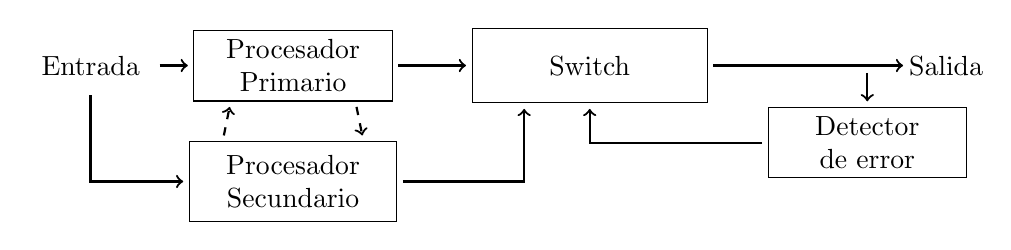
\begin{tikzpicture}[node distance=1cm, auto,]
  % definicion de estilos
  %Define style for boxes
   \tikzset{
   cuadro/.style={
           rectangle,
           draw=black,
           text width=6.5em,
           minimum height=2em,
           text centered},
    % Define arrow style
    arrow/.style={
           ->,
           thick,
           shorten <=2pt,
           shorten >=2pt,}	
    }
  \tikzstyle{circulo} = [draw, fill=black, circle, node distance=1cm, minimum size=5pt, inner 
sep=3pt]
    
  % Gráfico
  \node[inner sep=5pt] (entrada) {Entrada};
  \node[cuadro, right=0.5cm of entrada] (prim) {Procesador Primario};
  \node[cuadro, inner sep=5pt,below=0.5cm of prim] (secu) {Procesador Secundario};
  \node[cuadro, inner sep=10pt, right=1cm of prim] (selec) {Switch};
  \node[inner sep=0pt, right=2cm of selec](ghost1){};
  \node[cuadro, below=0.5cm of ghost1](detector) {Detector de error};
  \node[inner sep=0pt, right=0.5cm of ghost1] (salida) {Salida};
  
  \draw[arrow] (entrada)--(prim);
  \draw[arrow] (entrada)|-(secu);
  \draw[arrow, dashed] (prim.-30) -- (secu.30);
  \draw[arrow, dashed] (secu.150) -- (prim.-150);
  \draw[arrow] (prim)--(selec);
  \draw[arrow] (secu)-|(selec.-150);
  \draw[arrow] (detector)-|(selec);
  \draw[arrow] (selec)--(salida);
  \draw[arrow] (ghost1)--(detector);
 \end{tikzpicture}
 \caption{Representación del proceso pares}
 \label{fig:repPares}
\end{figure}

\end{comment}

\subsubsection{Diversidad de datos}
La diversidad es una técnica utilizada para mejorar la eficiencia en los checkpoint y restart, 
usando diferentes entradas por cada reinicio. Esto se basa en que las fallas en el 
\ac{SW} son dependientes de las entradas. Es poco probable que la misma falla se 
de con la misma secuencia de entrada \citep{FTDesign}.

\subsubsection{Bloques de recuperación}

Esta técnica combina las bases de la técnica de checkpoints y restart enfocada con múltiples 
versiones de un componente de \ac{SW} en el sentido de que una versión de \ac{SW} diferente es 
lanzada cada vez que se encuentra una falla. Los 
checkpoints son creados antes de que una versión de \ac{SW} se ejecuta.
La ejecución de las múltiples versiones pueden ser 
secuencial o paralelas dependiendo de la disponibilidad de la capacidad de procesamiento y 
perfomance requerida \citep{SoftwareFaultToleranceATutorial}.

%La representación de esta técnica se puede observar en el figura~[AGREGAR IMAGEN].
Las 
versiones son diferentes implementaciones de un mismo programa. Solo una de estas versiones provee 
la salida del sistema. Si un error es detectado por el test de aceptación, se vuelve hacia atrás, 
se retoma el último checkpoint, y se vuelve a ejecutar el módulo de \ac{SW} pero con una 
versión diferente a la que se ejecutó anteriormente \citep{FTDesign}.  	

Los checks del test de aceptación deben mantenerse simples para mantener la velocidad de la 
ejecución \citep{FTDesign}.

\begin{comment}
\begin{figure}[h]
 \centering
 \begin{tikzpicture}[node distance=1cm, auto,]
  % definicion de estilos
  %Define style for boxes
   \tikzset{
   cuadro/.style={
           rectangle,
           draw=black,
           text width=6.5em,
           minimum height=2em,
           text centered},
    % Define arrow style
    arrow/.style={
           ->,
           thick,
           shorten <=2pt,
           shorten >=2pt,}	
    }
       
  \tikzstyle{circulo} = [draw, fill=black, circle, node distance=1cm, minimum size=5pt, inner 
sep=3pt]
    
  % Gráfico
  \node[inner, sep=5pt] (input1){Entrada 1};
  \node[inner, sep=5pt, below=0.5cm of input1] (input2){Entrada 2};
  \node[inner, sep=5pt, below=0.5cm of input2] (puntos1){...};
  \node[inner, sep=5pt, below=0.5cm of puntos1] (inputn){Entrada n};
  \node[cuadro, right=0.5cm of input1] (version1){Versión 1};
  \node[cuadro, right=0.5cm of input2] (version2){Versión 2};
  \node[inner, sep=5pt, right=2cm of puntos1](puntos2){...};
  \node[cuadro, right=0.5cm of inputn] (versionn){Version n};
  
  \node[cuadro, above=1cm of version1] (check) {Memoria Checkpoint};
  \node[cuadro, right=1cm of version2] (switch) {Swith n a 1};
  \node[inner, sep=0pt, right=1cm of switch](ghost1){};
  \node[cuadro, below=0.5cm of ghost1](test){Test de aceptación};
  
  \node[inner, sep=0pt, right=0.5cm of ghost1](output){Salida};
 
  %Arrows
  \draw[arrow] (input1)--(version1);
  \draw[arrow] (input2)--(version2);
  \draw[arrow] (inputn)--(versionn);
  \draw[arrow] (version1)-|(switch.west);
  \draw[arrow] (version2)--(switch);
  \draw[arrow] (versionn)-|(switch.west);
  \draw[arrow] (ghost1)--(test);
  \draw[arrow] (switch)--(output);
  
  \draw[arrow, dashed] (check.-40) -- (version1.30);
  \draw[arrow, dashed] (version1.150) -- (check.-145);
  
  

 \end{tikzpicture}
 \caption{Configuración de bloques de recuperación}
 \label{fig:repPares}
\end{figure}
\end{comment}

%\subsubsection{Programación N-version}

%\subsubsection{Programación N-Auto Checking}


\chapter{Estado del arte}\label{chap:estado_del_arte}
\epigraph{Locura es hacer lo mismo una y otra vez esperando obtener resultados diferentes}{Albert Einstein}
% section that explain binary tree
\input{../Chapters/Art_State/Binary_tree/Binary_tree.tex}
% section that explain Distributed network
\section{Redes distribuidas}\label{sec:redes_distribuidas}
Una red de computadoras hace referencia a un conjunto de computadoras autónomas que se encuentran interconectadas, esto quiere decir que pueden intercambiar información \citep{Tanenbaum12}. Una red distribuida tiene como principal característica que no existe un nodo central que ``gestione'' toda la red. Todas las cargas de las tareas y/o actividades son distribuidas entre los nodos que forman parte de la red.

Una red distribuída es tolerante a fallas si los nodos pueden formar subredes \citep{Stivaros92}. Es decir, la red se debe mantener activa y conectada, con diferentes topologías e interconexiones, que permitan tolerar posibles fallas producidas en algunos nodos y permitir mantener la perfomance \citep{Stivaros92}. Debido a que el procesamiento de la red se encuentra distribuída en todo el sistema, esto brinda una ventaja por encima de los sistemas centralizados desde el punto de vista de la confiabilidad \citep{Pradhan82}. Un componente importante de las redes distribuidas tolerantes a fallas, es la topología del sistema \citep{Pradhan82}.

Siguiendo la notación de \cite{Pradhan82} para describir la topología del sistema se utiliza, un gráfico sin direccionamiento G = <V,E>, donde V representa un set de nodos y E representa un set de relaciones. \cite{Stivaros92} agrega que $V(G) = \{v_1,v_2,v_3, ... v_n \}$ representa un vector de nodos, los cuales tiene probabilidades de operación $P = (p_1, p_2, p_3, p_n)$; y define una función de asignación $\pi$, la cual es una función que asigna V con una probabilidad $P_{\pi(v)}$.

La \ac{FT} de la red G, dado el vector de probabilidades \vec{P} y una función de asignación $\pi$, tal como se viene discutiendo anteriormente, es la probabilidad de que la red continúe funcionando, es decir continúe conectada, aún en la falla (aleatoria) de alguno de sus nodos, esto se denota  como $FT(G;\vec{P},\pi)$.

Se dice que un subset de nodos S, es un estado tolerante a fallas del sistema G, cuando estos nodos se mantienen conectados y funcionales. Se utiliza $\theta$ para indicar el conjunto de todos los S posibles. Un estado tolerante S contribuye $\prod_{v\in S}{P_{\pi (v)}} \prod_{v \notin S} (1-p_{\pi (v)})$ a la probabilidad de \ac{FT}.

Para calcular el total de la \ac{FT} del sistema, incluyendo todo los S, se hace: $$FT(G;\vec{P};\pi) = \sum_{S \in \theta}{Pr(S)} = \sum_{S \in \theta}{\prod_{v\in S}{P_{\pi (v)}} \prod_{v \notin S} (1-p_{\pi (v)})}$$

Una relación entre nodos es representado  como ij, lo cual representa un enlace bidireccional entre nodos. El grado del nodo i representa el número de relaciones que inciden en ese nodo, el cual se escribe $d_i$. Así, $d_i$ está limitado por el número de puertos de entrada y salida disponibles por cada nodo \citep{Pradhan82}. $k_{ij}$ representa el número mínimo de \textit{hop} (hop representa la transmisión a través de un link de datos) \citep{Pradhan82}

\cite{Stivaros92} y \cite{Pradhan82} mencionan la existencia de varias topologías que pueden ser aplicadas en una red distribuida tolerante a fallas. Una topología estrella posee una baja distancia entre nodos, pero una pobre tolerancia a fallas (\citep{Pradhan82}; \citep{Stivaros92}). La topología anillo, permite un simple ruteo, pero existen grandes distancias internodo. Un sistema completamente interconectado, presenta buenas características tolerantes a fallas, pero tiene un alto costo \citep{Pradhan82}. \cite{Pradhan82} propone una topología para una arquitectura distribuida de comunicación. Esta es una topología robusta, y puede llegar a ser compleja a medida que aumentan los nodos.

\subsection{Algoritmo de ruteo}
Los algoritmos de ruteos son necesarios en el desarollo de una arquitectura tolerante a fallas y reconfigurable. Los algoritmos de ruteo se los pueden dividir en dos: \textit{algoritmo primario} y \textit{algoritmo alternativo}. El primero es utilizado cuando no hay fallas de nodos. Se deben mantener los caminos para llegar, correctamente, al nodo destino. El segundo se utiliza en la presencia de alguna falla, este requiere que sea capaz de detectar la presencia de fallas, para luego reconfigurar el sistema. Estos algoritmos deben ser simples y requerir una mínima cantidad de \ac{HW} y \ac{SW}.

Agregado a lo mencionado en el párrafo anterior, deben existir algoritmos de diagnóstico distribuido de fallas, basados en los algoritmos de ruteo \citep{Pradhan82}.

% section that explain Ethernet Network
\section{Redes Ethernet en aviónica}
TTEthernet es una tecnología de red de computadoras comercializada por TTTech Computertechnik AG para el desarrollo de aplicaciones seguras. SAE Internation\footnote{http://www.sae.org} estandarizó esta red como SAE AS6802. TTEthernet se basa en el Ethernet clásico, en el cual se pone énfasis en las características principales que deben respetarse en sistemas críticos, tales como latencias de mensajes determinísticos, presición de tiempo real, tolerancia a fallas \citep{Loveless15}.

El Ethernet clásico presenta ventajas, tales como su alta velocidad de transmisión de datos, flexibilidad, y su disponibilidad y bajo costo (ya que se trata de un componente COTS)\citep{Loveless15}, hacen deseable su aplicación en el área espacial.  fue utilizado en diferentes proyectos aeroespaciales y en misiones importantes tales como el Space Shuttler y la Estación Espacial Internacional (ISS) \citep{Loveless15}. A pesar de esto, el Ethernet no cumple con el determinismo requerido por las aplicaciones de tiempo real de un vehículo espacial. Por tal motivo, se desarrolla el sistema TTEthernet, el cual introduce un reloj de sincronización descentralizado, permitiendo la transmisión mensajes \ac{TT}. En este tipo de red, existe una herramienta de planning que asigna a cada dispositivo un intervalo de tiempo, en el cual puede utilizar para transmitir frames.

TTEtheret puede actuar en dos clases de tráfico, con el obejtivo de soportar diferentes niveles de cricticidad de mensajes.
\begin{itemize}
  \item Rate-Constrained (RC), en el cual se llevan algunas restricciones de tamaño y rate de transmisión de frames,
  \item Best-Effort (BE), el cual se comporta de manera similar que el Ethernet
\end{itemize}

Esta tecnología toma tanto interés que el Sistema de Exploración Avanzada (AES)\footnote{Del ingles, Advanced Exploration Systems} de la \ac{NASA}, lleva a cabo un proyecto denominado Avionics and Software (A&S)


\chapter{Análisis y desarrollo de arquitectura tolerante a fallas}\label{chap:analisis_desarrollo}
\epigraph{La raza humana necesita un desafío intelectual. Debe ser aburrido ser Dios y no tener nada que descubrir}{Stephen Hawking}
% section that make an introduction
\section{Introducción}
Los proyectos aeroespaciales emplean una arquitectura de aviónica que se denomina \textbf{federada}, en la cual cada computadora del sistema se diseña para que desarrolle una sola función específica \citep{Loveless15}. Esta estrategia de diseño tiene varias ventajas, por tal motivo ha sido utilizada a lo largo de los años. En contraposición, cuenta con varias desventajas, que alientan al surgimiento de nuevas formas de pensamiento y desarrollo de aviónica de sistemas espaciales. Algunas de estas desventajas que ya fueron mencionadas con anterioridad son la masa y una utilización ineficiente de los procesadores. Para ello se está comenzando a desarrollar arquitecturas con el paradigma IMA.


\chapter{Arquitectura propuesta}\label{chap:arquitectura_propuesta} 
\epigraph{Dadme un punto de apoyo y moveré el mundo}{Arquímedes} 
\section{Introducción}
Aquí hago la propuesta de la arquitectura.

El capítulo estará dividido en

\begin{itemize}
\item Arbol de requerimientos
\item Diseño estructural (Diagramas de bloques, bloques internos)
\item Diseño dinámico (Diagramas de secuencia, interacción, maquina de estados,)
  
\end{itemize}

\section{Árbol de requrimientos}
A continuación se detallas los requerimientos que van a guiar el diseño y
desarrollo de la propuesta de arquitectura de aviónica tolerantes a fallas
basada en componentes \ac{COTS} para satélites. En la Figura
\ref{fig:DiagramaRequerimientos} y en la Tabla \ref{table:Requerimientos} se pueden
observar los requerimientos. 

\begin{figure}[h!]
 \centering
 \includegraphics[scale=0.4]{images/Capitulo5/Diagrama_de_Requerimientos.JPG}
  \caption{Diagrama de requerimientos de la arquitectura propuesta}
\label{fig:DiagramaRequerimientos}
\end{figure} 

\begin{sidewaystable}[]
  \small
\centering
\caption{Tabla de requerimientos de la arquitectura propuesta}
\label{table:Requerimientos}
\begin{tabular}{|l|l|l|l|}
\hline
\multicolumn{1}{|c|}{\textbf{}} & \multicolumn{1}{c|}{\textbf{ID}} & \multicolumn{1}{c|}{\textbf{Name}} & \multicolumn{1}{c|}{\textbf{Detail}}                                                                           \\ \hline
0                               & L1\_001                          & L1\_001                            & The architecture components shall be Components Off-The-Shelf category                                         \\ \hline
1                               & L2\_000                          & L2\_000                            & The architecture shall be reconfigurate when a node fail.                                                      \\ \hline
2                               & L2\_001                          & L2\_001                            & Each subsystem shall represented for a Components Off-The-Shelf                                                \\ \hline
3                               & L1\_000                          & L1\_000                            & Shall be develop an avionics architecture for spacecraft using Components Off-The-Shelf                        \\ \hline
4                               & L1\_002                          & L1\_002                            & The architecture shall have at least 6 subsystems                                                              \\ \hline
5                               & L1\_003                          & L1\_003                            & The architecture shall have fault tolerance techniques to assurance the the mission life                       \\ \hline
6                               & L1\_004                          & L1\_004                            & The main bus to interconnect components shall be the Controller Area Network Bus developed for Bosch           \\ \hline
7                               & L1\_005                          & L1\_005                            & The architecture shall be sufficient to make a master degree thesis                                            \\ \hline
8                               & L2\_002                          & L2\_002                            & The architecture shall implements a based Controller Area Netoword protocol to intercommunicate the components \\ \hline
9                               & L3\_000                          & L3\_000                            & The intercommunication between nodes shall used the CANae protocol developed in the master degree thesis       \\ \hline
10                              & L1\_006                          & L1\_006                            & The architecture shall to assurance at least 10 years mission life                                             \\ \hline
11                              & L3\_001                          & L3\_001                            & The architecture shall use the distributed network philosophy                                                  \\ \hline
12                              & L1\_007                          & L1\_007                            & The thesis shall be finished in 1 year                                                                         \\ \hline
13 & L2\_003 & L2\_003 & The nodes shall send and receive message from any nodes connected to the architecture. \\ \hline
\end{tabular}
\end{sidewaystable}

A continuación se explica cada uno de los requerimientos:
\begin{itemize}
\item\textbf{L1\_000}: Este es el objetivo principal de la presente tesis:
  desarrollar una arquitectura de aviónica tolerante a fallas basada en
  componentes COTS para vehículos espaciales.
\item\textbf{L1\_001}: El principal requerimiento de este trabajo de tesis,
  es desarrollar una arquitectura basada en componentes COTS, lo cual agrega un
  grado importante de innovación tecnológica y complejidad, siendo de especial
  interés para INVAP trabajar con estos tipos de componentes.
\item\textbf{L1\_002}: Este requerimiento hace referencia que se debe asegurar
  el correcto funcionamiento de la arquitectura con una cantidad de al menos
  6 subsistemas.
\item\textbf{L1\_003}: Este requerimiento exige que la arquitectura sea
  tolerante a fallas para así poder sastifacer el requerimiento \textbf{L1\_006}.
\item\textbf{L1\_004}: Este requerimiento (constraint) indica que se debe pensar
  la arquitectura para ser utilizada con el bus CAN de Bosch. Este requerimiento
  es de interés par INVAP.
\item\textbf{L1\_005}: Este requerimiento indica que la arquitectura que se
  desarrolle debe ser sufiencite para lograr terminar una tesis de maestría. Por
  el diseño y desarrollo debe ser solo el suficiente y necesario para cumplir
  con el presente trabajo.
\item\textbf{L1\_006}: Este requerimiento indica que debe asegurarse que la
  arquitectura sea lo suficientemente robusta como para asegurar el el tiempo de
  vida de la misión de 10 años como mínimo. Existe un \textbf{problema} con este
  requerimiento, y es que para los alcances de esta tesis, será imposible
  verificar si se cumple con este requerimiento.
\item\textbf{L1\_007}: Este requerimiento indica que el trabajo de tesis tiene
  que ser finalizado en menos de un año. Esto tiene relación con el
  requerimiento \textbf{L1\_005} debido a que no se logrará alcanzar el detalle
  necesario para lograr la correcta implementación, verifación y validación de
  la arquitectura.
\item\textbf{L2\_000}: Este requerimiento exige que la arquitectura pueda
  reconfigurarse cuando un nodo falle.
\item\textbf{L2\_001}: Este requerimiento indica que para esta instancia de
  trabajo cada subsistema será tratado como un nodo dentro de la arquitectura.
\item\textbf{L2\_002}: Este requerimiento indica que se debe utilizar dentro de
  la arquitectura un protocolo de comunicación basado en el Bus CAN de Bosch.
\item\textbf{L2\_003}: Este requerimiento asegura que los nodos deben poder enviar
  y recibir mensajes de cualquier otro nodo conectado a la red CANae.
\item\textbf{L3\_000}: Este requerimiento indica que el protocolo de
  comunicación utilizado en esta arquitectura debe ser CANae. Este protocolo
  fue desarrollado en el presente trabajo de tesis (Vease:\ref{Appendix:A}).
\item\textbf{L3\_001}: Este requerimiento exige la utilización de una
  filosofía de red distribuída para su diseño y desarrollo.
\end{itemize}

\section{Casos de Uso}
A continuación se muestra el diagrama de Casos de Uso para la arquitectura propuesta.
Se observa que el único Actor identificado en esta instancia de desarrollo es
la aplicacción de usuario que se conecta a la arquitectura.  Dentro de esta
arquitectura propuesta se encuentra el protocolo de comunicación CANae.

\begin{figure}[h!]
 \centering
 \includegraphics[scale=0.6]{images/Capitulo5/Caso_de_Uso_Arquitectura.JPG}
  \caption{Diagrama de Casos de Uso de arquitectura propuesta}
\label{fig:DiagramaCUArqPropuesta}
\end{figure} 


%\chapter{Análisis y resultados}
%\section{Introdución}
Si llego a implementar algo (que no creo a esta altura) colocar aquí el código y los resultados.


\chapter{Conclusión}\label{chap:conclusiones}
\epigraph{Las personas que están lo suficientemente locos como para pensar que pueden cambiar el mundo, son los que lo hacen.}{Steve Jobs}
Estas son las putas conclusiones

%\input

%\include{secciones/AreaDeEstudio}
%\section*{Datos}
\label{sec:datos}
%\section*{Metodología}
\label{sec:metodologia}
%\include{secciones/Resultados}
%\include{secciones/Discusion}

% ----------------------------------------------------------------------------------------------

\newpage
\nocite{*}
\bibliography{biblio.bib}
%\bibliographystyle{plainnatesp.bst}
%\bibliographystyle{apacite}
\bibliographystyle{apa-emma.bst}
\addcontentsline{toc}{chapter}{Bibliograf\'ia}

%------------------------------------------------------------------------------
% EN CASO DE TENER APÉNDICES, DESCOMENTAR A CONTINUACIÓN
\appendix
% CANae
\chapter{Protocolo de comunicación: CANae 0.1 Alpha Version}\label{Appendix:A}
% introducción
\section{Introducción}
En este apéndice se explica el diseño de la versión Alpha del protocolo CANae. Este protocolo se basa en el la capa de aplicación del protocolo CAN y CANopen. El nombre CANae proviende de la unión de CAN y CONAE. 

\subsection{Revisiones}
\begin{table}[H]
  \centering
  \caption{Revisiones de CANae}
  \label{table:revisiones_canae}
  \begin{tabular}{|p{1cm}|p{2cm}|p{2cm}|p{5cm}|}
  \hline
  \multicolumn{1}{|c|}{\textbf{Ver.}} & \multicolumn{1}{c|}{\textbf{Who.}} & \multicolumn{1}{c|}{\textbf{When}} & \multicolumn{1}{c|}{\textbf{What}} \\ \hline \hline
 $0.1$ Alpha & Emmanuel Arias & 25/06/2017 & Initial Version \\ \hline
  \end{tabular}
\end{table}
\newpage


% Capa de aplicación
\input{Secciones/Protocolo_Comunicacion/Capa_Aplicacion.tex}
% CMS
\section{CMS}
CMS ofrece un ambiente orientado a objeto para diseñar aplicaciones de usuario. CMS ofrece a la aplicación la posibilidad de modelar su comportamiento en la forma de objeto. Este elemento de servicio ofrece variables, eventos que se utilizan para diseñar y especificar cómo la funcionalidad de un módulo puede acceder a las interfaces CAN.

El servicio asume que no hay fallas provenientes de la capa de enlace de datos y la capa física de la red CAN. Las fallas, si ocurren, son resueltas por el NMSE (Network Management Service Element).

\subsection{Prioridades de los objetos}
La arbitración del protocolo CAN se realiza teniendo en cuenta la prioridad de los identificadores de los frames que se envía. La arbitración es no destructiva, debido a la necesidad de tener un procesamiento de mensajes de tiempo real. La prioridad se determina teniendo en cuenta cada uno de los bits. El indentificador de los objetos y eventos de CMS está compuesto por 8 bits más 3 bits que los diferenciará entre objetos y eventos. Los eventos tiene mayor prioridad.

\begin{tabular}{lll}
    000 & (ID) & Tipo de evento \\
    111 & (ID) & Prioridad objeto \\
\end{tabular}

La prioridad de los objetos es un UInteger de 1 byte. La prioridad más baja es 0 y la prioridad más alta de 1. Por lo tanto la prioridad va desde 00000000b (mayor prioridad) hasta 11111111b (menor prioridad).

\subsection{Objeto CMS}
Un objeto CMS define una estructura de dato que se debe respetar para poder enviar información (variables) a través de la red. El objeto está compuesto por los siguientes campos:
\begin{itemize}
   \item Name: string de 6 caracteres (6 bytes)
   \item User\_type: \{client, server\} (1 bit)
   \item Priority: UInteger (1 bytes)
   \item Datatype: UInteger identificador del tipo de datos (1 byte)
   \item Data: Indefinido.
\end{itemize}

\begin{figure}[h!]
 \centering
 \includegraphics[scale=0.4]{images/Secciones/AppendixA/CMSObject.JPG}
  \caption{Definición del Objeto CMS}
\label{fig:CMSObject}
\end{figure} 

\subsection{Servicios de CMS}
Con respecto a las variables de CMS existen una serie de servicios brindados por CMS, que pueden ser tanto \textit{local services} como \textit{remote services}. Su clasificación depende de si se está accediendo a variables almacenadas dentro del nodo, o bien se está intentando acceder (escribir o leer) una variable remota. Un evento está definido de la siguiente manera:

\begin{itemize}
   \item Name: string de 6 caracteres (6 bytes)
   \item User\_type: \{client, server\} (1 bit)
   \item Priority: UInteger (1 bytes)
   \item Event\_Type: UInteger identificador del tipo de datos (1 byte)
   \item Data: Indefinido.
\end{itemize}


\subsubsection{Servicios locales}
\begin{itemize}
  
\item Boolean define\_variable(String name, DataType data\_type)
  \begin{itemize}
  \item \textbf{String name}: Nombre de la variable.
    \item \textbf{DataType data\_type}: Tipo de dato de la variable. 
  \end{itemize}
  
\item Boolean set\_variable(String name, UInteger destination, Data data, UInteger priority)
  \begin{itemize}
    \item \textbf{String name}: Nombre de la variable.  
    \item \textbf{UInteger destination}: Direción del destinatario. Esta dirección debe ser provista por el NMT.
    \item \textbf{Data data}: Datos a enviar.
    \item \textbf{UInteger priority}: Prioridad de la variable.
  \end{itemize}
  
\item Boolean update\_variable(String name, data data)
  \begin{itemize}
    \item \textbf{String name}: Nombre de la variable
    \item \textbf{Data data}: Datos a enviar    
  \end{itemize}
 
\end{itemize}
\subsubsection{Servicios remotos}
\begin{itemize}
\item Boolean write\_variable(String name, Data data)
  \begin{itemize}
    \item \textbf{String name}: Nombre de la variable a escribir
    \item \textbf{Data data}: Dato a escribir
  \end{itemize}
\item Data read\_variable(String name)
  \begin{itemize}
    \item \textbf{String name}: Nombre de la variable a leer
  \end{itemize}
\end{itemize}

\subsection{Eventos}
Los eventos se utilizan para modelar comportamientos asíncronos, tales como temperatura excedida en un tiempo determinado. La ocurrencia de los eventos es detectada por el nodo, que en ese momento actuará como server y se notifica a todos los clientes.
\begin{comment}
\begin{figure}[h!]
 \centering
 \includegraphics[scale=0.4]{images/Secciones/AppendixA/CMSEvent.JPG}
  \caption{Definición del Objeto CMS}
\label{fig:CMSEvent}
\end{figure} 
\end{comment}
Los servicios al igual que las variables se dividen en servicio local o servicio remoto. Los servicios se describen a continuación.

\subsubsection{Servicios locales}
\begin{itemize}
\item define\_event(String name, UInteger priority, UInteger event\_type)
  \begin{itemize}
  \item \textbf{String name}: Nombre del evento
  \item \textbf{UInteger priority}: Prioridad del evento
  \item \textbf{UInteger event\_type}: Tipo de evento según tabla \ref{table:prioridad_eventos}
  \end{itemize}

\end{itemize}

\subsubsection{Servicios remotos}

\begin{itemize}
\item Event notify\_event()
\item Boolean store\_event(String name)
  \begin{itemize}
    \item \textbf{String name}: Nombre de evento a almacenar
  \end{itemize}
  
\item Event read\_event(String name)
  \begin{itemize}
    \item \textbf{String name}: Nombre de la variable a leer
  \end{itemize}
\end{itemize}

\subsubsection{Prioridad de eventos}
La prioridad de los eventos se define como una tabla que se define al momento de implementar el protocolo. Al desarrollar la tabla de prioridades se debe cuidar la relevancia de los eventos. La prioridad más baja es 0. El tamaño de la prioridad del evento es de 1 byte. Por lo tanto la prioridad va desde 00000000b (mayor prioridad) hasta 11111111b (menor prioridad).

\begin{table}[h!]
  \centering
  \caption{Prioridad eventos}
  \label{table:prioridad_eventos}
  \begin{tabular}{|l|l|l}
    \cline{1-2}
    00000000 & Nombre evento & Mayor prioridad \\\cline{1-2}
    00000001 & Nombre evento & \\\cline{1-2}
    00000010 & Nombre eevnto & \\\cline{1-2}
    ... & ... & ... \\\cline{1-2}
    11111111 & Nombre evento & Menor prioridad \\\cline{1-2}
  \end{tabular}    
\end{table}

Esta tabla de prioridad de eventos, debe ir acompañada de un diccionario de eventos, donde se almacena los datos relevantes al evento. En esta se hace una descripción del evento. Sirve de guía para la implementación y desarrollo de aplicaciones que identifican eventos.

El diccionario debería incluir los siguientes campos:
\begin{itemize}
\item Nombre del evento
\item Descripción del evento
\item Prioridad
\item Umbral límite inferior (En el caso de que existiera)
\item Umbral límite superior (En el caso de que existiera)
\end{itemize}




% NMT
\section{NMT}\label{Appendix:A}
Esta es una entidad de la capa de aplicación que permite el correcto
funcionamiento de la red. Esta entidad tiene los servicios necesarios para que
cada nodo tenga un conocimiento de todos los nodos conectados en la red. Esto
permite el armado de una tabla de nodos, que es mantenida en todo los
nodos. Esta entidad exige la existencia de un nodo monitor, que es el encargado
de monitorear y configurar la red. Luego, una vez en funcionamiento este nodo
monitor no será vital para la red. En el NMT se deben implementar los
algoritmos de ruteo. El entorno NMT se puede observar en la Figura \ref{fig:NMT}

\begin{figure}[h!]
 \centering
 \includegraphics[scale=0.4]{images/Secciones/AppendixA/NMT.JPG}
  \caption{Definición de la entidad NMT}
\label{fig:NMT}
\end{figure} 

Por medio de este servicio es posible conocer el estado de la red CAN. Los
mensajes de NMT CAN son envíados con máxima prioridad. 
\subsection{Objectos NMT}
El Network Management utiliza tres objetos diferentes para modelar una red CAN.
\begin{itemize}
 \item \textbf{Network Object}: Representa todos los modulos conectados en la
  red CAN. El objeto de red existe en todos los nodos.
 \item \textbf{Remote Node Object}: Cada nodo conectado a la red CAN tiene
   representado todos los demás nodos.    
 \item \textbf{Node Object}: Cada nodo que es gestionado por el servicio NMT
   está representado por un node object. Este objeto se encuentra modelado en
   cada uno de los nodos.    
 \end{itemize}
Cada nodo y su objeto (remoto y local) es unívocamente identificado en la red
por su NMT Address. Esta dirección no se puede cambiar. Esto significa que por
cada nodo existe un objeto nodo y un objeto nodo remoto con el mismo NMT
Address, replicada en todos los nodos de la red. 

\subsection{Servicios NMT}
La entidad NMT ofrece los siguientes servicios:
\subsubsection{Module Control Service}
EL NMT monitor incializa los nodos NMT que forman parte de la red CAN
distribuida, a través de este servicio se asegura que todos los nodos se
encuentran configurados y funcionando correctamente.
\subsubsection{Error Control Services}
Através de este servicio, el NMT detecta fallas en la red CAN, ya sea fallas
producidas en la capa de enlace de datos (fallas locales) y/o fallas
producidos en otros nodos.
\subsubsection{Configuration Control Services}
Através de este servicio se realiza la configuarción de la red.

\subsubsection{Servicios a implementar}
La funciones típicas que se deben implementar en el NMT son los siguientes:
\begin{itemize}
\item Boolean create\_network()
\item Boolean create\_remote\_network() 
\item Boolean remove\_remote\_network()
\item Boolean create\_node(UInteger Node-ID, UInteger address, String description)
  \begin{itemize}
  \item \textbf{UInteger Node-ID}: ID del nodo a crear.
  \item \textbf{UInteger address}: Dirección del nodo creado. UInteger entre [0,255]
  \item \textbf{String description}: Descripción del nodo.
  \end{itemize}
\item Boolean delete\_node(UInteger Node-ID)
  \begin{itemize}
   \item \textbf{UInteger Node-ID}: Dirección del nodo a eliminar. UInteger entre [0,255]
  \end{itemize}
    
\item UInteger identify\_remote\_node(UInteger Node-ID)
  \begin{itemize}
  \item \textbf{UInteger Node-ID}: Dirección del nodo a idetenficar
  \end{itemize}

\item UInteger identify\_node()
  
\item Boolean connect\_node()
  
\item Boolean connect\_remote\_node(UInteger Node-ID)
  \begin{itemize}
    \item \textbf{UInteger Node-ID}: ID del nodo remoto a conectar.
  \end{itemize}

\item Boolean prepare\_node()
\item Boolean prepare\_remote\_node(UInteger Node-ID)
  \begin{itemize}
   \item \textbf{UInteger Node-ID}: ID del nodo a pasar a modo preparado
  \end{itemize}
\item Boolean start\_node()
\item Boolean start\_remote\_node(UInteger Node-ID)
  \begin{itemize}
    \item \textbf{UIntenger Node-ID}: ID del nodo que comenzará a participar en la red.
   \end{itemize}
\item Boolean disconnect\_node()
\item Boolean disconnect\_remote\_node(UInteger Node-ID)
  \begin{itemize}
    \item \textbf{UInteger Node-ID}: ID del nodo a desconectar.
  \end{itemize}
\end{itemize}

\subsection{Protocolos NMT}
\subsubsection{Crear red CANae}
Para conectar correctamente la red CANae se debe respetar el protocolo NMT para crear la red.
En primer lugar el nodo monitor debe enviar el mensaje \textit{create\_remote\_network()}
para avisar a todos los nodos que deben crear sus propias instancias de
\textit{NetworkObject} a través de \textit{create\_network()}. Automáticamente, los nodos deben crear una propia instancia del nodo mediante
\textit{create\_node()}. Luego el nodo monitor envía el mensaje de
\textit{prepare\_remote\_node()} para prepara todos los nodos a conectarse a la red CANae.
Luego el nodo monitor envía la señal de \textit{connect\_remote\_node(UInteger Node-ID)} con
la dirección de todos los nodos que figuran en su \textit{NodeTableConfiguration}
preprogramada.
Luego cada nodo, correctamente preparado, se conecta a la red a través de
\textit{connect\_node()}.

Este protocolo puede ser observado en la Figura \ref{fig:ProtocolNMTConnectNet}
\begin{figure}[h!]
 \centering
 \includegraphics[scale=0.4]{images/Secciones/AppendixA/Protocol_NMT.JPG}
  \caption{Protocolo NMT}
  \label{fig:ProtocolNMTConnectNet}
\end{figure} 

\subsubsection{Crear Red}\label{NMT:crear_red}
Para lograr la correcta conexión de los nodos a la red, estos deben
configurarse. Cuando se alimenta la red, los nodos deben iniciar en estado de
\textit{escucha} esperando la orden del nodo monitor de crear la red mediante
\textit{create\_remote\_network()}. Esta se envía en broadcast a todos los nodos
conectados. Cuando el controlador de la capa de aplicaciónr recibe el mensaje
através del servicio NMT, este manda un mensaje al gesto del nodo interno, el
cual crea la \textit{tabla de configuración del nodo} y acutizaliza con la
información necesaria.

\begin{figure}[h!]
 \centering
 \includegraphics[scale=0.4]{images/Secciones/AppendixA/Create_Network.JPG}
  \caption{Crear Red}
  \label{fig:ProtocolNMTConnectNet}
\end{figure} 

\subsubsection{Crear Objecto Red, Objeto Nodo y Objeto Nodo Remoto}
Antes de comenzar a funcionar la red, cada nodo debe crear un objeto de red
exigidos por el protocolo NMT. Una vez que el proceso Crear Red termina,
el Gestor de la capa de Aplicación envía un mensaje \textit{create\_node()}
al Gestor del Nodo. El Gestor de Nodo crea un \textit{Network Object}. Este a su
vez crea un \textit{Node Object} y un \textit{Remote Node Object}. Estos objetos
pertenecen a la entidad NMT.

\begin{figure}[h!]
 \centering
 \includegraphics[scale=0.4]{images/Secciones/AppendixA/create_node.JPG}
  \caption{Crear Objecto Red, Objeto Nodo y Objeto Nodo Remoto}
  \label{fig:ProtocolNMTConnectNet}
\end{figure}































































































































































































































% DBT
\section{DBT}\label{Appendix:DBT}
DBT es



% Especificación de casos de uso
\chapter{Especificación de Casos de Uso}\label{Appendix:UseCase}

%%%%%%%%%%%%%%%%%%%%%%%%%%%%%%%
% Caso de uso: Enviar mensaje %
%%%%%%%%%%%%%%%%%%%%%%%%%%%%%%%

\section{Enviar Mensaje}

\large\textbf{Use Case ID}
\vspace{3mm}

El ID del Caso de eso es ARQ001

\Large\textbf{Historia del Caso de Uso}
\vspace{3mm}

\large\textbf{Creado por}
\vspace{3mm}

Arias Emmanuel

\large\textbf{Fecha de Creación}
\vspace{3mm}

12 de Junio del 2017

\large\textbf{Última actualización}
\vspace{3mm}

N/A

\large\textbf{Fecha de la última actualización}
\vspace{3mm}

N/A


\Large\textbf{Definición del Caso de Uso}
\vspace{3mm}

\large\textbf{Actor}
\vspace{3mm}

\textit{UserApplication}. Este la aplicación del usuario que se encuentra ejecutandose en el nodo.

\large\textbf{Descripción}
\vspace{3mm}

Este caso de uso recibe los mensajes que la aplicación de usuario necesita enviar
por la red hacia otro nodo en el sistema.

\large\textbf{Precondición}
\begin{itemize}
\item El nodo debe estar funcional y conectado a la red.
\item El protocolo CANae debe haber finalizado su inicialiación.
\item El nodo destino tiene que estar funcional.
\end{itemize}

\large\textbf{Postcondición}
\begin{itemize}
\item Debe asegurarase el correcto envío del mensaje.
\end{itemize}

\large\textbf{Prioridad}
\vspace{3mm}

Prioridad media.

\large\textbf{Curso normal de eventos}
\vspace{3mm}

El caso de uso recibe el mensaje proveniente de la aplicación
del usuario. En el siguiente paso prepara el mensaje siguiendo
los lineamientos del protocolo CANae. Por último lo envía a las
capas inferiores para ser enviado a través del protocolo CAN.

\large\textbf{Cursos alternativos}
\vspace{3mm}

N/A

\large\textbf{Excepciones}
\vspace{3mm}

En caso de producirse un error en el caso de uso, se lleva a cabo
una excepción, para avisar a la aplicación de usuario que se
produjo un error. 

\large\textbf{Includes}
\vspace{3mm}

N/A

\large\textbf{Notas y problemas}
\vspace{3mm}

N/A



%%%%%%%%%%%%%%%%%%%%%%%%%%%%%%%%
% Caso de uso: Recibir Mensaje %
%%%%%%%%%%%%%%%%%%%%%%%%%%%%%%%%

\section{Recibir Mensaje}

\large\textbf{Use Case ID}
\vspace{3mm}

El ID del Caso de eso es ARQ002

\Large\textbf{Historia del Caso de Uso}
\vspace{3mm}

\large\textbf{Creado por}
\vspace{3mm}

Arias Emmanuel

\large\textbf{Fecha de Creación}
\vspace{3mm}

12 de Junio del 2017

\large\textbf{Última actualización}
\vspace{3mm}

N/A

\large\textbf{Fecha de la última actualización}
\vspace{3mm}

N/A

\Large\textbf{Definición del Caso de Uso}
\vspace{3mm}

\large\textbf{Actor}
\vspace{3mm}

\textit{UserApplication}. Este la aplicación del usuario que se encuentra ejecutandose en el nodo.

\large\textbf{Descripción}
\vspace{3mm}

Este caso de uso recibe los mensajes proveniente de las capas inferiores de CAN
y luego es enviado a la aplicación del usuario.

\large\textbf{Precondición}
\begin{itemize}
\item El mensaje tiene que llegar sin errores.
\item El nodo debe estar conectado y funcional en la red.
\item El nodo debe estar preparada (no ocupado) para recibir el mensaje.
\end{itemize}

\large\textbf{Postcondición}
\vspace{5mm}

N/A

\large\textbf{Prioridad}
\vspace{3mm}

Prioridad media.

\large\textbf{Curso normal de eventos}
\vspace{3mm}

El caso de uso recibe el mensaje proveniente de las capas inferiores del CAN.
Se suponen que llegan sin errores. Luego se envía a la aplicación de usuario.

\large\textbf{Cursos alternativos}
\vspace{3mm}

N/A

\large\textbf{Excepciones}
\vspace{3mm}

N/A

\large\textbf{Includes}
\vspace{3mm}

N/A

\large\textbf{Notas y problemas}
\vspace{3mm}

N/A



%%%%%%%%%%%%%%%%%%%%%%%%%%%%%%%%%
% Caso de uso: Procesar Mensaje %
%%%%%%%%%%%%%%%%%%%%%%%%$%%%%%%%%

\section{Procesar Mensaje}

\large\textbf{Use Case ID}
\vspace{3mm}

El ID del Caso de eso es ARQ003

\Large\textbf{Historia del Caso de Uso}
\vspace{3mm}

\large\textbf{Creado por}
\vspace{3mm}

Arias Emmanuel

\large\textbf{Fecha de Creación}
\vspace{3mm}

12 de Junio del 2017

\large\textbf{Última actualización}
\vspace{3mm}

N/A

\large\textbf{Fecha de la última actualización}
\vspace{3mm}

N/A

\Large\textbf{Definición del Caso de Uso}
\vspace{3mm}

\large\textbf{Actor}
\vspace{3mm}

N/A

\large\textbf{Descripción}
\vspace{3mm}

Este caso de uso se encarga de recibir los mensajes desde la aplicación
de usuario y de las capas inferiores de CAN, para realizar un procesamiento.
Este procesamiento incluye empaquetado y desempaquetado, y verificación de
la ocurrencia de errores, clasificación de mensajes que contienen datos
o eventos.

\large\textbf{Precondición}
\begin{itemize}
\item El nodo debe estar conectado y funcional en la arquitectura.
\end{itemize}

\large\textbf{Postcondición}
\vspace{5mm}

N/A

\large\textbf{Prioridad}
\vspace{3mm}

Prioridad alta.

\large\textbf{Curso normal de eventos}
\vspace{3mm}

El caso de uso recibe el mensaje proveniente de las capas inferiores del CAN.
Se suponen que llegan sin errores. Se desempaqueta, se clasifica (si es datos
o evento) y luego se envía a la aplicación de usuario.

\large\textbf{Cursos alternativos}
\vspace{3mm}

N/A

\large\textbf{Excepciones}
\vspace{3mm}

N/A

\large\textbf{Includes}
\vspace{3mm}
Ver Rutear Mensajes. \ref{uc:RutearMensajes}

\large\textbf{Notas y problemas}
\vspace{3mm}

N/A


%%%%%%%%%%%%%%%%%%%%%%%%%%%%%%%%
% Caso de uso: Rutear Mensajes %
%%%%%%%%%%%%%%%%%%%%%%%%$%%%%%%%

\section{Rutear Mensaje}\label{uc:RutearMensajes}

\large\textbf{Use Case ID}
\vspace{3mm}

El ID del Caso de eso es ARQ003.1

\Large\textbf{Historia del Caso de Uso}
\vspace{3mm}

\large\textbf{Creado por}
\vspace{3mm}

Arias Emmanuel

\large\textbf{Fecha de Creación}
\vspace{3mm}

12 de Junio del 2017

\large\textbf{Última actualización}
\vspace{3mm}

N/A

\large\textbf{Fecha de la última actualización}
\vspace{3mm}

N/A

\Large\textbf{Definición del Caso de Uso}
\vspace{3mm}

\large\textbf{Actor}
\vspace{3mm}

N/A

\large\textbf{Descripción}
\vspace{3mm}

Este es el encargado de rutear los mensajes. Debe indicar que nodos intermedios
debe pasar el mensaje hasta llegar al nodo destino.

\large\textbf{Precondición}
\begin{itemize}
\item El nodo debe estar conectado y funcional en la arquitectura.
\item El mensaje debe estar clasificado y empaquetado.
\item Se debe conocer el nodo destino. 
\end{itemize}

\large\textbf{Postcondición}
\vspace{5mm}

N/A

\large\textbf{Prioridad}
\vspace{3mm}

Prioridad alta.

\large\textbf{Curso normal de eventos}
\vspace{3mm}

Este caso de uso una vez que se clasifica y empaqueta el mensaje,
debe consultar al Caso de Uso \textit{Gestion de Red} para verificar
que nodos intermedios debe pasar el mensaje hasta llegar al nodo
destino. 

\large\textbf{Cursos alternativos}
\vspace{3mm}

N/A

\large\textbf{Excepciones}
\vspace{3mm}

N/A

\large\textbf{Includes}
\vspace{3mm}

N/A

\large\textbf{Notas y problemas}
\vspace{3mm}

N/A


%%%%%%%%%%%%%%%%%%%%%%%%%%%%%%
% Caso de uso: Gestionar Red %
%%%%%%%%%%%%%%%%%%%%%%%%$%%%%%

\section{Gestionar Red}\label{uc:GestionarRed}

\large\textbf{Use Case ID}
\vspace{3mm}

El ID del Caso de eso es ARQ004

\Large\textbf{Historia del Caso de Uso}
\vspace{3mm}

\large\textbf{Creado por}
\vspace{3mm}

Arias Emmanuel

\large\textbf{Fecha de Creación}
\vspace{3mm}

12 de Junio del 2017

\large\textbf{Última actualización}
\vspace{3mm}

N/A

\large\textbf{Fecha de la última actualización}
\vspace{3mm}

N/A

\Large\textbf{Definición del Caso de Uso}
\vspace{3mm}

\large\textbf{Actor}
\vspace{3mm}

N/A

\large\textbf{Descripción}
\vspace{3mm}

Este caso de uso se encarga de gestionar la red. Se vale de las
bondades ofrecidas por CANae para conocer cuales son los nodos
conectados a la red y la distancia que existe entre el nodo
objetivo y el destino. 

\large\textbf{Precondición}
\begin{itemize}
\item El nodo debe estar conectado y funcional en la arquitectura.
\item El protocolo CANae debe haber finalizado su inicialización.
\item El protocolo CANae tiene que haber realizar la tabla de ruteo.
\end{itemize}

\large\textbf{Postcondición}
\vspace{5mm}

N/A

\large\textbf{Prioridad}
\vspace{3mm}

Prioridad alta.

\large\textbf{Curso normal de eventos}
\vspace{3mm}

El caso de uso utiliza las bondades del protocolo CANae para conocer
cuales son los nodos conectados a la red y su distancia. Este caso
de uso es la base para que se realice una correcta gestión de tareas
a realizar en el sistema. Luego con esto se pueden dividir las tareas que
se llevarán a cabo el los diferentes nodos de la red. 

\large\textbf{Cursos alternativos}
\vspace{3mm}

N/A

\large\textbf{Excepciones}
\vspace{3mm}

N/A

\large\textbf{Includes}
\vspace{3mm}

Ver Gestionar Tareas \ref{uc:GestionarTareas}

\large\textbf{Notas y problemas}
\vspace{3mm}

N/A


%%%%%%%%%%%%%%%%%%%%%%%%%%%%%%%%%
% Caso de uso: Gestionar Tareas %
%%%%%%%%%%%%%%%%%%%%%%%%%%%%%%%%%

\section{Gestionar Tareas}\label{uc:GestionarTareas}

\large\textbf{Use Case ID}
\vspace{3mm}

El ID del Caso de eso es ARQ004.1

\Large\textbf{Historia del Caso de Uso}
\vspace{3mm}

\large\textbf{Creado por}
\vspace{3mm}

Arias Emmanuel

\large\textbf{Fecha de Creación}
\vspace{3mm}

12 de Junio del 2017

\large\textbf{Última actualización}
\vspace{3mm}

N/A

\large\textbf{Fecha de la última actualización}
\vspace{3mm}

N/A

\Large\textbf{Definición del Caso de Uso}
\vspace{3mm}

\large\textbf{Actor}
\vspace{3mm}

N/A

\large\textbf{Descripción}
\vspace{3mm}

Este caso de uso se encarga de gestionar las tareas que se deben
ejecutar en la red. Para ello debe implementarse un algoritmo que
asegure la correcta comunicación con los nodos para lograr
la gestión de tareas del sistema.

\large\textbf{Precondición}
\begin{itemize}
\item El nodo debe estar conectado y funcional en la arquitectura.
\item El protocolo CANae debe haber finalizado su inicialización.
\item El protocolo CANae tiene que haber realizar la tabla de ruteo.
\end{itemize}

\large\textbf{Postcondición}
\vspace{5mm}

N/A

\large\textbf{Prioridad}
\vspace{3mm}

Prioridad alta.

\large\textbf{Curso normal de eventos}
\vspace{3mm}

En primer lugar debe consultar la tabla de ruteo para conocer la posción de los nodos.
Con ello y lista de tareas del sistema, lleva a cabo un algoritmo de
gestión de tareas, donde se negocia con los demás nodos que tareas se
van a llevar a cabo en los diferentes nodos.

\large\textbf{Cursos alternativos}
\vspace{3mm}

N/A

\large\textbf{Excepciones}
\vspace{3mm}

N/A

\large\textbf{Includes}
\vspace{3mm}

Ver Dividir Tareas \ref{uc:DividirTareas}

\large\textbf{Notas y problemas}
\vspace{3mm}

N/A


%%%%%%%%%%%%%%%%%%%%%%%%%%%%%%%
% Caso de uso: Dividir Tareas %
%%%%%%%%%%%%%%%%%%%%%%%%%%%%%%%

\section{Dividir Tareas}\label{uc:DividirTareas}

\large\textbf{Use Case ID}
\vspace{3mm}

El ID del Caso de eso es ARQ004.1.1

\Large\textbf{Historia del Caso de Uso}
\vspace{3mm}

\large\textbf{Creado por}
\vspace{3mm}

Arias Emmanuel

\large\textbf{Fecha de Creación}
\vspace{3mm}

12 de Junio del 2017

\large\textbf{Última actualización}
\vspace{3mm}

N/A

\large\textbf{Fecha de la última actualización}
\vspace{3mm}

N/A

\Large\textbf{Definición del Caso de Uso}
\vspace{3mm}

\large\textbf{Actor}
\vspace{3mm}

N/A

\large\textbf{Descripción}
\vspace{3mm}

Este caso de uso se encarga de realizar al división de las tareas,
una vez que se ha llevado a cabo la negociación.

\large\textbf{Precondición}
\begin{itemize}
\item El nodo debe estar conectado y funcional en la arquitectura.
\item El protocolo CANae debe haber finalizado su inicialización.
\item El protocolo CANae tiene que haber realizar la tabla de ruteo.
\item Se debe haber llevado a cabo la negociación correctamente.
\end{itemize}

\large\textbf{Postcondición}
\begin{itemize}
  \item Se actualiza la lista de tareas en los nodos.
\end{itemize}
\large\textbf{Prioridad}
\vspace{3mm}

Prioridad alta.

\large\textbf{Curso normal de eventos}
\vspace{3mm}

Luego de recibir el resultado de la negociación, actualiza la lista
de tareas que se llevan a cabo en los nodos. E informa a los demás nodos.

\large\textbf{Cursos alternativos}
\vspace{3mm}

N/A

\large\textbf{Excepciones}
\vspace{3mm}

N/A

\large\textbf{Includes}
\vspace{3mm}

N/A

\large\textbf{Notas y problemas}
\vspace{3mm}

N/A


%%%%%%%%%%%%%%%%%%%%%%%%%%%%%%%
% Caso de uso: Dividir Tareas %
%%%%%%%%%%%%%%%%%%%%%%%%%%%%%%%

\section{Dividir Tareas}\label{uc:DividirTareas}

\large\textbf{Use Case ID}
\vspace{3mm}

El ID del Caso de eso es ARQ004.1.1

\Large\textbf{Historia del Caso de Uso}
\vspace{3mm}

\large\textbf{Creado por}
\vspace{3mm}

Arias Emmanuel

\large\textbf{Fecha de Creación}
\vspace{3mm}

12 de Junio del 2017

\large\textbf{Última actualización}
\vspace{3mm}

N/A

\large\textbf{Fecha de la última actualización}
\vspace{3mm}

N/A

\Large\textbf{Definición del Caso de Uso}
\vspace{3mm}

\large\textbf{Actor}
\vspace{3mm}

N/A

\large\textbf{Descripción}
\vspace{3mm}

Este caso de uso se encarga de realizar al división de las tareas,
una vez que se ha llevado a cabo la negociación.

\large\textbf{Precondición}
\begin{itemize}
\item El nodo debe estar conectado y funcional en la arquitectura.
\item El protocolo CANae debe haber finalizado su inicialización.
\item El protocolo CANae tiene que haber realizar la tabla de ruteo.
\item Se debe haber llevado a cabo la negociación correctamente.
\end{itemize}

\large\textbf{Postcondición}
\begin{itemize}
  \item Se actualiza la lista de tareas en los nodos.
\end{itemize}
\large\textbf{Prioridad}
\vspace{3mm}

Prioridad alta.

\large\textbf{Curso normal de eventos}
\vspace{3mm}

Luego de recibir el resultado de la negociación, actualiza la lista
de tareas que se llevan a cabo en los nodos. E informa a los demás nodos.

\large\textbf{Cursos alternativos}
\vspace{3mm}

N/A

\large\textbf{Excepciones}
\vspace{3mm}

N/A

\large\textbf{Includes}
\vspace{3mm}

N/A

\large\textbf{Notas y problemas}
\vspace{3mm}

N/A


%%%%%%%%%%%%%%%%%%%%%
% Caso de uso: FDIR %
%%%%%%%%%%%%%%%%%%%%%

\section{FDIR}\label{uc:FDIR}

\large\textbf{Use Case ID}
\vspace{3mm}

El ID del Caso de eso es ARQ005

\Large\textbf{Historia del Caso de Uso}
\vspace{3mm}

\large\textbf{Creado por}
\vspace{3mm}

Arias Emmanuel

\large\textbf{Fecha de Creación}
\vspace{3mm}

12 de Junio del 2017

\large\textbf{Última actualización}
\vspace{3mm}

N/A

\large\textbf{Fecha de la última actualización}
\vspace{3mm}

N/A

\Large\textbf{Definición del Caso de Uso}
\vspace{3mm}

\large\textbf{Actor}
\vspace{3mm}

N/A

\large\textbf{Descripción}
\vspace{3mm}

Este caso de uso se encarga de la detección, aislación
y recuperación de errores que se produzcan tanto en el nodo
como en la red.

\large\textbf{Precondición}
\begin{itemize}
\item El nodo debe estar conectado y funcional en la arquitectura.
\item El protocolo CANae debe haber finalizado su inicialización.
\item El protocolo CANae tiene que haber realizar la tabla de ruteo.
\end{itemize}

\large\textbf{Postcondición}
\begin{itemize}
\item Se toma una medida para lograr aislar y recuperar la arquitectura
  del error que se ha producido.
\end{itemize}
\large\textbf{Prioridad}
\vspace{3mm}

Prioridad alta.

\large\textbf{Curso normal de eventos}
\vspace{3mm}

Este caso de uso debe observar como se encuentra la red en cada momento. Para
ello hace uso de las bondades que le puede brindar el caso de uso \textit{
  Gestionar Red}. Cuando detecta que se ha producido una falla en el nodo o en la red,
lanza una excepción para manejar el problema. 

\large\textbf{Cursos alternativos}
\vspace{3mm}

Ver \textit{Reconfigurar Arquitectura} \ref{uc:ReconfigurarArquitectura}

\large\textbf{Excepciones}
\vspace{3mm}

N/A

\large\textbf{Includes}
\vspace{3mm}

N/A

\large\textbf{Notas y problemas}
\vspace{3mm}

No se llega a realizar un diseño y desarollo de este caso de uso
en esta instancia del trabajo de tesis.


%%%%%%%%%%%%%%%%%%%%%%%%%%%%%%%%%%%%%%%%%%
% Caso de uso: Reconfigurar Arquitectura %
%%%%%%%%%%%%%%%%%%%%%%%%%%%%%%%%%%%%%%%%%%

\section{Reconfigurar Arquitectura}\label{uc:ReconfigurarArquitectura}

\large\textbf{Use Case ID}
\vspace{3mm}

El ID del Caso de eso es ARQ006

\Large\textbf{Historia del Caso de Uso}
\vspace{3mm}

\large\textbf{Creado por}
\vspace{3mm}

Arias Emmanuel

\large\textbf{Fecha de Creación}
\vspace{3mm}

12 de Junio del 2017

\large\textbf{Última actualización}
\vspace{3mm}

N/A

\large\textbf{Fecha de la última actualización}
\vspace{3mm}

N/A

\Large\textbf{Definición del Caso de Uso}
\vspace{3mm}

\large\textbf{Actor}
\vspace{3mm}

N/A

\large\textbf{Descripción}
\vspace{3mm}



\large\textbf{Precondición}
\begin{itemize}
\item El nodo debe estar conectado y funcional en la arquitectura.
\item El protocolo CANae debe haber finalizado su inicialización.
\item El protocolo CANae tiene que haber realizar la tabla de ruteo.
\end{itemize}

\large\textbf{Postcondición}
\begin{itemize}
\item Se toma una medida para lograr aislar y recuperar la arquitectura
  del error que se ha producido.
\end{itemize}
\large\textbf{Prioridad}
\vspace{3mm}

Prioridad alta.

\large\textbf{Curso normal de eventos}
\vspace{3mm}

Este caso de uso debe observar como se encuentra la red en cada momento. Para
ello hace uso de las bondades que le puede brindar el caso de uso \textit{
  Gestionar Red}. Cuando detecta que se ha producido una falla en el nodo o en la red,
lanza una excepción para manejar el problema. 

\large\textbf{Cursos alternativos}
\vspace{3mm}

Ver \textit{Reconfigurar Arquitectura} \ref{uc:ReconfigurarArquitectura}

\large\textbf{Excepciones}
\vspace{3mm}

N/A

\large\textbf{Includes}
\vspace{3mm}

N/A

\large\textbf{Notas y problemas}
\vspace{3mm}

No se llega a realizar un diseño y desarollo de este caso de uso
en esta instancia del trabajo de tesis.

% Antecedentes
\chapter{Antecedentes}\label{Appendix:Antecedentes}

El objetivo de este apéndice es que el lector conozca el crecimiento de las investigaciones
llevadas a cabo en el área de estudio de la presente tesis. Esto ayudará a comprender
y respaldar las motivaciones del presente trabajo.
Así, se podrá demostrar que existe una gran cantidad de investigadores
(los cuales se incrementan con el paso de los años), que se enfocan en la problemática a las cuales
se enfrenta esta tesis. Para ello, se utilizó la base de datos Scopus\footnote{www.scopus.com}, la cual es una
base de datos que contiene abstracts, citaciones, y artículos científicos. 

En primer lugar se realizó la búsqueda de las palabras claves ``COTS satellites'', obteniendo los resultados
que se muestran en la Figura \ref{fig:ant1}. Se observa que existe una tendencia creciente en las investigaciones
que contienen estas \textit{key words}.
Se encontró una cantidad total de 2047 artículos científicos. 

\begin{figure}[h!]
 \centering
 \includegraphics[scale=0.8]{images/Secciones/antecedentes/Cantidad_paper-COTS-Satellite.png}
  \caption{Cantidad de investigaciones con palabra clave ``COTS satellite''}
\label{fig:ant1}
\end{figure}

Por otro lado, se llevó a cabo una búsqueda de las mismas palabras claves, pero esta vez,
la consulta se realizó para conocer los principales países involucrados en estas investigaciones.
De esto, se obtiene el gráfico de la Figura \ref{fig:ant2}. Como se observa el país con más
investigaciones es Estados Unidos.

\begin{figure}[h!]
 \centering
 \includegraphics[scale=0.6]{images/Secciones/antecedentes/Cantidad_paper-COTS-Satellite-Country.png}
  \caption{Cantidad de investigaciones con palabra clave ``COTS satellite'' por países}
\label{fig:ant2}
\end{figure}

De la misma manera se realizó una consulta de las palabras claves: ``Fault Tolerance Satellite'',
para conocer tanto la cantidad de artículos existentes (Figura \ref{fig:ant3}). Nuevamente, se puede
observar un creciente interés en llevar a cabo investigaciones con respecto a las áreas de interés
de este trabajo de tesis. 

\begin{figure}[h!]
 \centering
 \includegraphics[scale=0.8]{images/Secciones/antecedentes/Cantidad_paper-fault_tolerance_satellite.png}
  \caption{Cantidad de investigaciones con palabra clave ``Fault Tolerance Satellite''}
\label{fig:ant3}
\end{figure}


Luego se realizó una búsqueda con las siguientes \textit{key words}: ``COTS Fault Tolerance''. Como resultado se obtuvo que existe una lateralización en la tendencia de las investigaciones en estas
áreas como se puede observar en la Figura \ref{fig:ant4}. Nuevamente, el país con más investigaciones
en el área sigue siendo Estados Unidos \ref{fig:ant5}. 


\begin{figure}[h!]
 \centering
 \includegraphics[scale=0.6]{images/Secciones/antecedentes/Cantidad_paper-COTS_fault_tolerance.png}
  \caption{Cantidad de investigaciones con palabra clave ``COTS Fault Tolerance'' }
\label{fig:ant4}
\end{figure}


\begin{figure}[h!]
 \centering
 \includegraphics[scale=0.5]{images/Secciones/antecedentes/Cantidad_paper-COTS_fault_tolerance-Country.png}
  \caption{Cantidad de investigaciones con palabra clave ``COTS Fault Tolerance'' por países}
\label{fig:ant5}
\end{figure}

Por último se llevó a cabo una consulta con las palabras claves: ``Fault Tolerance Satellite
Architecture''. Los resultados se pueden observar en las Figuras \ref{fig:ant6} y \ref{fig:ant7}.
Como en las consultas anteriores, se observa un creciente interés por el estudio de esta área de
trabajo y el país como mayor publicación, sigue siendo Estados Unidos.



\begin{figure}[h!]
 \centering
 \includegraphics[scale=0.8]{images/Secciones/antecedentes/Cantidad_paper-fault_tolerance_satellite_architecture.png}
  \caption{Cantidad de investigaciones con palabra clave ``Fault Tolerance Satellite Architecture'' }
\label{fig:ant6}
\end{figure}


\begin{figure}[h!]
 \centering
 \includegraphics[scale=0.4]{images/Secciones/antecedentes/Cantidad_paper-fault_tolerance_satellite_architecture-Country.png}
  \caption{Cantidad de investigaciones con palabra clave ``Fault Tolerance Satellite Architecture'' por países}
\label{fig:ant7}
\end{figure}

De estas búsquedas sencillas, se puede llegar a la conclusión de que en general, existe una tendencia
creciente en investigaciones en el área que compete este trabajo de tesis. Además, se puede
obtener como conclusión de que existe una mayor cantidad de investigaciones en la dirección de
``COTS'' y ``Satellites''. Esto se puede justificar con la existencia de una necesidad de
reducir costos a la hora de la fabricación de satélites.

Por otro lado, lo que resulta interesante (o más bien preocupante) es que no hay una
tendencia creciente, en las investigaciones sobre ``COTS'' y ``Fault Tolerance''
que acompañe a lo dicho en el párrafo anterior. Esto puede traer consecuencias negativas
para aquellos que traten de desarrollar vehículos satelitales con componentes COTS, y no
cuenten con estrategias de tolerancia a fallas.



\begin{comment} 
\newpage
$\ $
\thispagestyle{empty} % para que no se numere esta pagina
\newpage
$\ $
\thispagestyle{empty}
\end{comment}
\end{document}
